%
% The Current Maintainer of this work is Paul Vojta.

\documentclass[phd]{ucbthesis}
\usepackage{biblatex}
\usepackage{color}
\usepackage{graphicx}
\usepackage{subcaption}
\usepackage{siunitx}
\usepackage{listings}
\usepackage{rotating}
\usepackage{multirow}
\usepackage{xspace}
\usepackage{amsmath}


% To compile this file, run "latex thesis", then "biber thesis"
% (or "bibtex thesis", if the output from latex asks for that instead),
% and then "latex thesis" (without the quotes in each case).

% Double spacing, if you want it.  Do not use for the final copy.
\def\dsp{\def\baselinestretch{2}\large\normalsize}
%\dsp


% If the Grad. Division insists that the first paragraph of a section
% be indented (like the others), then include this line:
% \usepackage{indentfirst}

% commands
\newcommand{\ignore}[1]{}
\newcommand{\TODO}[1]{{\color{red}\textbf{TODO: #1}}}
\newcommand{\RISCV}{\mbox{RISC-V}}
\newcommand{\wunits}[2]{\mbox{#1\,#2}}

% Environments
\newenvironment{widequote}%
               {\list{}{\leftmargin=0.3in\rightmargin=0.3in}\item[]}%
               {\endlist}

% commands use to alias tbd names
% Paper name
\newcommand{\PNAME}{\mbox{\textsc{fased}}\xspace}
% Simulation framework name
\newcommand{\SIMNAME}{MIDAS\xspace}

\bibliography{refs}

% Increase the depth of numbering sections

\hyphenation{Rocket-Chip MIDAS}
\begin{document}

% Declarations for Front Matter

\title{FPGA-Accelerated Simulation of ASICs with Dynamically Scaling Clocks}
\author{David Thomas Biancolin}
\degreesemester{Spring}
\degreeyear{2019}
\degree{Doctor of Philosophy}
\chair{Professor Krste Asanovi\'c}
\cochair{Adjunct Professor Jonathan Richard Bachrach}
\othermembers{Professor Sanjit Seshia \\ Professor Robert Leachman }
% Previous degrees are no longer to be listed on the title page.
% \prevdegrees{B.A. (University of Northern South Dakota at Hoople) 1978 \\
%   M.S. (Ed's School of Quantum Mechanics and Muffler Repair) 1989}
\field{Electrical Engineering and Computer Science}
% Designated Emphasis -- this is optional, and rare
% \emphasis{Colloidal Telemetry}
% This is optional, and rare
% \jointinstitution{University of Western Maryland}
% This is optional
\campus{Berkeley}

% For a masters thesis, replace the above \documentclass line with
% \documentclass[masters]{ucbthesis}
% This affects the title and approval pages, which by default calls this
% document a "dissertation", not a "thesis".

% A slightly modified template of the ms thesis to reuse the title variables
\clearpage
%\input{tex/cover}
\maketitle
% Delete (or comment out) the \approvalpage line for the final version.
%\approvalpage
\copyrightpage
% (Optional) \part{First Part}

\begin{abstract}
%While specialization appears to be only path towards higher performance and more
energy efficient computer hardware, the enormous non-recurring engineering (NRE) cost
of designing modern systems-on-a-chip~(SoCs) is a major barrier to the wider
adoption of custom silicon. As part of a larger effort exploring more
cost-effective agile methodologies for designing custom silicon, this work
contributes to a novel \emph{single-FPGA} hardware emulation framework, FireSim, that aims to
radically reduce the cost of doing fast and accurate full-system simulation.

In this dissertation, we start by introducing a compiler infrastructure, called
\texttt{Golden Gate}, capable of performing general multi-cycle resource
optimizations in order to fit larger SoCs on a single FPGA. The
nature of these optimizations is described at length in A. Magyar's
dissertation~\cite{MagyarDissertation}. Using this compiler infrastructure, we
study optimization-compatible schemes for simulating SoCs with more realistic
clocking organizations.  We first present a simple approach for simulating
systems with multiple fixed-frequency clocks.  We then extend this to support a
more general class of clock switching and generation behavior, notably to
enable timing-exact simulation dynamic frequency scaling. Our approach is based
on prior work in software-based, conservative parallel-discrete event
simulation wherein we replace clock switching and generation structures, like
clock multiplexors, with decoupled models that act on timestamped message
streams.  Unlike other academic FPGA-based systems, which tend to be FPGA
prototypes that rely on direct instantiation of FPGA clocking primitives, here
we strictly use clock gating to derive simulated clocks, making our approach
far easier to use and FPGA portable.

\end{abstract}

\begin{frontmatter}
% You can delete the \clearpage lines if you don't want these to start on
% separate pages.

\setcounter{tocdepth}{2}
\setcounter{secnumdepth}{2}
\tableofcontents
\clearpage
\listoffigures
\clearpage
\listoftables
\begin{acknowledgements}
\end{acknowledgements}
\end{frontmatter}

\pagestyle{headings}


%\chapter{Introduction}
%
%%Today, the semiconductor industry finds itself in the midst of a storm emerging
from two colliding fronts\footnote{I borrow this metaphor from my advisor,
Krste Asanovi\'c.}. The first
of these, the hot front, is an exponential growth in the diversity and volume
of computing applications.  While AI, specifically machine
learning, has captured the zeitgiest, advances in semiconductor process
technologies have made it possible to embed computing in nearly all aspects of
human life. This manifests at the extremes as deeply embedded systems, often running in highly
energy-constrained environments, and cloud-hosted services, running in
multi-megawatt-scale datacenters, all interconnected via an evermore capable internet.  All of
this---from the smallest embedded microcontrollers to the largest
datacentered-oriented servers, and the networking hardware that connects
them---runs on transistor technologies whose fundamental physics have not
changed since the mid-twentieth century.

Indeed, the ``cold" front of this storm is the inevitable slowing of transistor
scaling trends that have long been the hallmark of the semiconductor industry.
First, we lost Dennard scaling~\cite{DennardScaling}: a regime in which a
shrink in transistor channel length and voltage would produce a proportional
reduction in the delay of a circuit built from them.  Dennard scaling drove an
era of exponential increase in computing performance wherein one could simply
reimplement an existing design in the latest process technology to realize
large speedups. Dennard scaling ended in the mid-aughts when it became
difficult to further  scale transitor voltages without losing the ability to
shut them off~\cite{ScalingChallenges}, forcing power density to increase. This
put a thermal limit on how fast one could clock a chip and led microprocessor
manufacturers to abandon development of higher-frequency, deeply pipelined
machines.

In the years since, advances in computing performance have ridden on the back
of the industry's better-known scaling trend, Moore's Law~\cite{MooresLaw}. Even if
transistors were not getting faster, they were still shrinking. These extra
transistors could be translated into larger caches and prediction structures,
physically wider vector and SIMD intruction pipelines, and most notably, more
processor cores. In this time, we also saw the rise of the general-purpose
GPU~(GPGPU), whose more parallel architecture scales naturally to use more
transistors than a conventional microprocessor. GPGPUs have been
a fundamental driver in the success of many modern machine-learning
techniques~\cite{AlexNet}.  Unfortunately, GPGPUs are far from truly
general-purpose; the bulk of the world's applications still run on conventional
microprocessors where improvements offered by more cores and other
microarchitectural enchanchments are bearing less fruit.

With no radically better general-purpose computer architecture (based in
silicon or otherwise) waiting in the wings, there is broad agreement that only means to deliver continued advances in
computing performance and energy efficiency is with specialization. In
academia, many researchers are building accelerators
for specific application domains, like graph computing~\cite{Graphicionado}
and machine learning~\cite{Eyeriss}. In industry, there is a growing number of
companies designing there own silicon where previously they would have
purchased offerings from existing players. Notable
examples include Tesla~\cite{FSDChip}, Amazon~\cite{Graviton},
Google~\cite{TPU}, and mostly recently, Apple\footnote{Apple has long been
designing its own SoCs for its mobile phones, but used Intel SoCs in their laptops and desktops.} with their M1
SoC~\cite{AppleM1}.

What this ``specialization" should look like is the defining question
of this era of computer architecture research. However, the more narrow concern of
this dissertation is how a particular microarchitecture should be implemented in silicon.  While
application-specific integrated circuits (ASICs), offer the best potential for
realizing these improvements, the non-recurring engineering~(NRE) cost of a new
design is enormous and growing~(Figure~\ref{fig:chip-nre}). As a result, reconfigurable logic devices like
field-programmable gate arrays~(FPGAs) have long filled low-volume niches where
the NRE of custom silicon~(i.e., an ASIC) cannot be effectively amortized. The need for
lower cost, energy-efficient hardware has also driven a resurgance in
structured ASICs~\cite{SAHARA}: these are FPGA-like devices whose
field-programability has been removed. Structured ASICS attempt to close the performance and
energy-efficiency gap between FPGAs and ASICs while saving up to 90 \% of the
NRE of an equivalent ASIC~\cite{StructuredASIC}.  Nonetheless, we believe the
performance and energy-efficiency costs~\cite{FPGAGap2} of using these
intermediate technologies is large enough to justify a redoubled effort to make
standard-cell-based ASIC design more economical.

The large NRE of developing an ASIC is in part historical.  Years of
advantagenous scaling trends have bred a business model into the industry in
which, at least in advanced technologies, relatively few unique designs are
taped out in enormous volumes. Simultaenously, advances in general-purpose computers dissuaded
investment in smaller-volume custom-silicon projects: why, after all, would one
design an ASIC, when one could wait two years for the next Intel CPU?
As a result, tools and metholodogies have been designed and optimized around
large NREs and large volumes to amortize them. Moreover, the established
players in the electronic design automation~(EDA) industry, responsible for
developing the tools used to design ASICs, are exceptionally profitable and have little short-term
incencitive to alter this business model. For the benefits of custom silicon to be attainable for
the non-Apples and Googles of the world this will need to change.

\begin{figure}
    \centering
    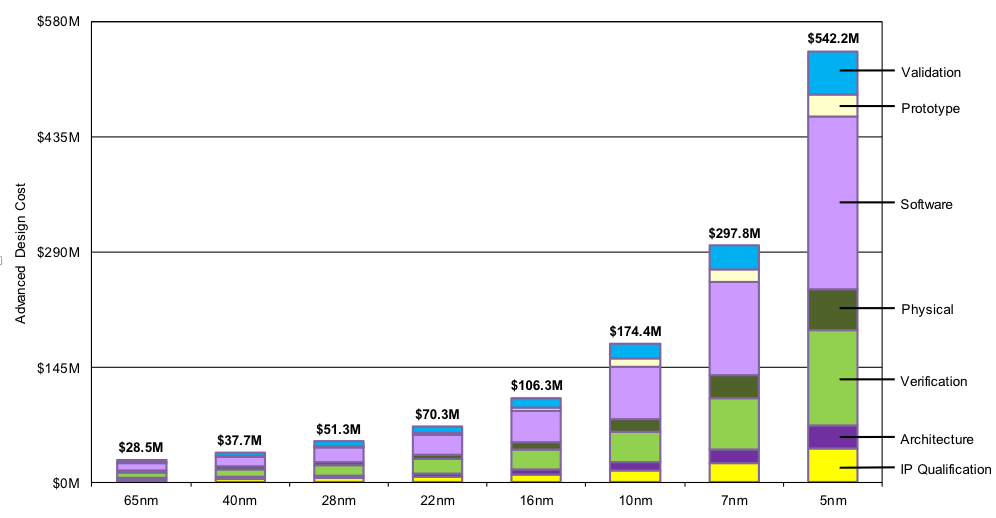
\includegraphics[width=0.99\textwidth]{figures/nre-cost.png}
    \caption{Early design non-recurring engineering~(NRE) cost
    at various feature dimensions. Source: IBS.}
    \label{fig:chip-nre}
\end{figure}

Part of the problem is that there appears to be no silver bullet for reducing
ASIC NRE, as there many disparate sources that often span multiple domains of
chip design~(Figure~\ref{fig:chip-nre}). Instead, we will need many diverse
tooling improvements united under a reimagined methodology for building custom
silicon. At Berkeley, we have articulated one such vision inspired by agile
software-engineering practises~\cite{AgileHW} and have built tools to support it.
These tools include Chisel~\cite{Chisel}, a more productive hardware-design
language (HDL) based in Scala, and FIRRTL~\cite{FIRRTL}, a flexible
intermediate representation for hardware that makes it easier to build
compilers. Perhaps the largest contribution to this vision has been the RISC-V
instruction set architecture~(ISA)~\cite{WatermanDissertation}.  Being open and
free-to-use, RISC-V enables chip designers to build customized microprocessors
while extending an open-source software toolchain.  This avoids the costs and
legal encumbarances of using a priopreitary ISA, or the massive engineering
burden of developing a fully custom ISA. RISC-V adoption has been meteoric in
recent years, both in academia outside of Berkeley~\cite{BlackParrot, Celerity,
Pulp}, and in industry, where a growing body of companies, notably SiFive,
Western Digital, and Nvidia have been developing new RISC-V implementations.

One unaddressed deficiency in chip design that drives verification, validation and software development
costs, is the lack of a good full-system simulation technology. Ideally, such
a technology would be:
\begin{itemize}
    \item \textbf{Fast.} As fast as silicon prototype, so as to enable running full system
    stacks and complete applications.
\item \textbf{Detailed.} It would simulate SoC's timing characteristics exactly.
\item \textbf{Productive.} It would be easy to debug and fast to recompile.  It would feel much like a software-based simulator.
\item \textbf{Inexpensive.} It would be cheap to deploy so that it could be made widely accessible
        to hardware and software design teams and support running large parallel experiments.
\end{itemize}

In practise, existing simulation technologies are forced to prioritize two of
these objectives. Software simulators, despite being easy to use and relatively
inexpensive, are much too slow to run full-system simulations when providing a
cycle-accurate model of the chip. For speed, chip designers are forced to turn
to hardware acceleration, in the form of FPGA prototyping and hardware
emulation.  Of the two, FPGA prototypes tend to be faster and less expensive,
and so see extensive use in software development and regression testing later
in the design cycle.  Conversely, hardware emulation is slower and considerably
more expensive, but offers a software-simulator-like debugging experience that
makes it a critical tool for pre-silicon verification. We will expand more on these
differences in Chapter~\ref{sec:simulation-background}.

The central question of the simulation work underway at Berkeley asks if it is
possible to build a simulation platform that can marry the speed of FPGA
prototyping, and the productivity of hardware emulation, while being radically
cheaper to deploy. Such a technology would put hardware emulation in the hands
of smaller research groups, and make it more widely available in companies
where scarse emulation resources must be carefully scheduled. Additionally, if
it is fast enough, it could subsume the role of a conventional FPGA prototype,
reducing the engineering burden of having parallel emulation and FPGA
prototyping infrastructures. If this technology is going to be inexpensive, two
things are clear.  First, it must use commericial off-the-shelf~(COTS) FPGA
platforms, and not custom devices or system integration as is true of all
commerical emulators. Second, this technology's software ecosystem, including
tools and IP libraries, will need to be open-source with the hope that they can
be developed and maintained by a community of users instead of a private team
of engineers.

This is no small undertaking but one made easier by recent technology trends.
Firstly, modern FPGAs are enormous, continue to be amoung the greatest
beneficiaries of Moore's law since they can naturally scale to use larger
transistor budgets. Advances in multi-die integration technologies have made
it easier to reliably manufacture even larger FPGAs. This makes it possible to
simulate considerably larger systems on a single FPGA.  Secondly, FPGAs are now available
in public cloud and provided by many major vendors like Amazon Web Services~\cite{amazonf1}.
This means a team can avoid the expense of building and
maintaining their own local FPGA cluster, and can use newer FPGAs as they
become available. Cloud services also provide an elastic supply of FPGAs,
allowing users to scale out experiments as needed, instead of needing to
provision a local cluster for the worst case. While the rates of using
cloud-based FPGAs are currently non-trivial, we expect these to fall in the
future as the costs of these services are amortized. Finally, it would be
difficult to build out an emulation infrastucture without the aforementioned advances in
open-source tooling. A compiler lies at the heart of all hardware emulation systems:
FIRRTL and its and Scala-based compiler infrastructure provide flexible
abstractions for translating a design into an FPGA-hosted emulator. FPGA-hosted emulation
infrastucture requires customized hardware, and more productive hardware-design
languages, like Chisel, makes it considerably easier for a small team to build
it. Finally, for an open-source infrastructure to see use, it
requires open-source input designs to both encourage adoption and inform
development. Here, we can leverage a growing body of RISC-V based processors,
such as Rocket~\cite{RocketChip} and BOOM~\cite{BOOM}, to feed into our system.

While it initially began as a project to study warehouse-scale computers, the
FireSim~\cite{FireSim} project has been our attempt at building out this
new technology. FireSim has been the basis for a
number of emulation-related research papers at Berkeley: we have studied
detailed DRAM timing models~\cite{FASED}, non-invasive, full-system profiling
techniques~\cite{FirePerf}.  FireSim-adjacent projects, using the same
underlying compiler, MIDAS~\cite{MIDAS}, have explored novel techniques for rapid
debugging~\cite{DESSERT}, and energy estimation~\cite{Simmani, Strober}. Over
time, features from these projects have gradually been integrated in mainline
FireSim, where they are employed by a growing user base.

Unfortunately, limitations with MIDAS limited its scope
to simple designs. First, these designs were small: they could be directly
implemented on a single Xilinx Ultrascale+ VU9P FPGA. In contrast, FPGA prototypes
of modern SoCs require partitioning over multiple FPGAs~\cite{FPMM}.  Second, these systems possessed only a single
clock domain. Conversly, modern SoCs have dozens of clocks whose frequencies
may change during execution. Without the ability to simulate
even a small number of fixed-frequency clocks it was difficult to get truly
accurate performance estimates with FireSim. Addressing these two challenges
drove the design of a new optimizing-compiler called Golden Gate~\cite{GoldenGate}.

To simulate larger systems, Golden Gate uses multi-cycle resource optimizations
to replace FPGA-hostile blocks. Golden Gate automates many techniques
deployed in prior academic work in FPGA-accelerated microarchitecture
simulation to radically improve the capacity of single FPGA. These
optimizations are the focus of Albert Magyar's dissertation~\cite{MagyarDissertation}.
Addressing the second challenge of simulating systems with more realistic clock
organizations is the subject of this dissertation. The contribution of this
work are threefold:

\begin{enumerate}
\item We describe Golden Gate, an optimizing compiler infratructure to deploy module-based
    multi-cycle resource optimizations~(Chapter~\ref{sec:golden-gate}. This
    contribution is shared with Albert Magyar, and is also described in his
    dissertation.

\item A simple, FPGA-flexible, extension to Golden Gate to support systems
    with fixed frequency clocks that is compatible with multi-cycle resource optimizations~(Chapter~\ref{sec:static-multiclock}).

\item A general, distributed approach for simulating clock generating and switching structures,
    based off of  prior work in software parallel discrete-event
    simulation~(Chapter~\ref{sec:dynamic-multiclock}). As above, our
    implementation co-exists with all multi-cycle resource
    optimizations.
\end{enumerate}

All of the software described in this dissertation is open source. We make
frequent reference to specific versions of the FireSim codebase to provide more
context in each chapter. Code references will use \texttt{monospace typeface}
where applicable. We hope this will help document features of FireSim as more
users adopt it. At time of writing, Golden Gate and support for fixed-frequency
clocks~(Chapter~\ref{sec:static-multiclock}) have been integrated into mainline
FireSim and are under active use. The features described in
Chapter~\ref{sec:dynamic-multiclock} are tagged \texttt{pdes}, and will be
merged in the future.

\section{Previous Publication, Collaboration, and Funding}

Portions of this work were published at the 2019 International Conference on
Computer-Aided Design as ``Golden Gate: Bridging The Resource-Efficiency Gap
Between ASICs and FPGA Prototypes'', though in this dissertation we focus on
the design of the compiler. The specific resource optimization employed in that
publication is described at length in Albert Magyar's dissertation~\cite{MagyarDissertation}.  Early results
from our initial support for emulation of multiple fixed-frequency
phase-aligned clocks, were published as ``Accessible, Resource-Efficient
FPGA-Accelerated Emulation Using FireSim'' in a July 2021 IEEE MICRO special
issue on FPGAs in Computing.

Donggyu Kim drove the bulk of MIDAS development based on his work on
Strober~\cite{Strober}. In the ``1.0" version of MIDAS presented in his
dissertation~\cite{DGKDissertation}, I contributed the design of endpoint
system. The final version of that compiler used by FireSim is described in
Chapter~\ref{sec:fpga-des}.

The work uses features developed by other FireSim contributors. Notable
contributors include Alon Amid, who developed much of the debug infrastructure,
Howard Mao, who has contributed to nearly all subsystems in FireSim, and Sagar
Karandikar, who ported MIDAS to use AWS and designed the cloud manager.

Finally, Golden Gate was the product of a tight collaboration between myself
and Albert Magyar. Much of the complexity in our dissertations is tied to the
FIRRTL-based software instructure required to analyze target SoCs and transform
them into latency-insensitive networks. This common infrastructure is described
at length in Chapter~\ref{sec:golden-gate}, and is the basis for the remainder
of the disseration.

The information, data, or work presented herein was funded in part by the
Advanced Research Projects Agency-Energy (ARPA-E), U.S. Department of Energy,
under Award Number DE-AR0000849.  Research was partially funded by ADEPT Lab
industrial sponsors and affiliates Intel, Apple, Futurewei, Google, and
Seagate.  The views and opinions of authors expressed herein do not necessarily
state or reflect those of the United States Government or any agency thereof.



\chapter{Anatomy Of A Modern SoC}

% in this section we review the design of a modern SOC with particular focus on
% it's clocking and reset structures, to motivate the design of our simulation
% infrastructure described later in this dissertation.

% Intro paragraph: Leave to introduction.
% - Talk about size
%  - 2.5 - 3D integration
%  - Give examples of large GPUs, CPUs
% - Heterogeneity
%   - Talk about specialization
%
% Combination of enormous size and increasing heterogenity leads to more complex
% clocking structures. Jump into this section assuming this has been established.
%

%  Overview of clock use in a modern SoC
%  - GALs
%  - Example SoC (eagle)
% Section: Clock domain crossings
% - Metastability, synchronizer chains
% - Fully asynchronous crossings
% - Rational crossings
% - Other types; see Ben Keller
% Section: Clock generation and selection structures
% - Clock Muxes
% - Clock Dividers
% - PLLs and DLLs
% Section: Reset sequences
% - How does a chip come out of reset, how do the clocks come up. Ordering considerations.
% Section: Clock gating
% Section: Dynamic frequency scaling
% - Explain what and why (DVFS)
% - Refer back to previous section RE: how clocks are reconfigured
% - Given an example system from Berkeley
% - Study an example system from not berkeley
% Clocks and EDA
% - SDC


\chapter{Full-System Simulation of SoCs}

Full-system simulation is used ubiquitously in SoC design and verification. We commence this chapter
with an exploration of the roles served by full-system simulation
in the SoC design process, and discuss commonly used full-system
simulation technologies with emphasis on hardware-accelerated forms like FPGA
prototyping and hardware emulation. From there we pivot to study how computer
architecture researchers employ full-system simulation to conduct higher-level
architectural and microarchitectural studies, and how academics have sought to
use FPGAs to accelerate these simulations.
We conclude the chapter by reviewing work done by the Berkeley Architecture
Research~(BAR) group over the past decade that attempts to build more
cost-effective hardware emulators by applying techniques from these
FPGA-accelerated microarchitecture simulators as automatic transformations to
SoC RTL.

To avoid confusion when speaking of computers simulating computers, the
literature commonly makes a distinction between the \emph{target}, the system
being simulated, and the \emph{host}, the system
executing the simulation. The host is often not a single machine but
a collection of interconnected machines, which may include CPUs,
GPUs, and FPGAs.

\section{A Tour of Full-System Simulation for SoC Design}

Simulation is central to performing three fundamental tasks of SoC design.

\begin{enumerate}

    \item \textbf{Prototyping:} ``What thing should we
        build?" Prototyping serves as a means to rapidly evaluate different
        design points with an imperfect model of a proposed design.

    \item \textbf{Verification:} ``Did we build the thing right?" Verification
        serves to check, or prove, that a particular implementation
        correctly executes.

    \item \textbf{Validation:} ``Did we build the right thing?" Validation
        serves to show that the implementation fulfills the objectives set out
        for the system.

\end{enumerate}

Both prototyping and verification can be applied at all levels of the design
hierarchy.  For example, given a specification of the system into which an
accelerator is integrated, one could prototype different design points and
verify an implementation of that accelerator. Validation, however, seeks to
answer a system-level question that spans the entire computing stack.  The
surest way to validate a system is not in simulation, but at-speed with a
physical prototype or the final product itself. However, waiting for a silicon
prototype pushes validation late into the design cycle making it challenging or
impossible to pivot the design of the system based on validation results. To
perform \emph{pre-silicon} validation, a fast and accurate full-system
simulator is required.

Here, SoC designers are confronted with a fidelity-performance-cost trade-off,
and are forced to use multiple different simulation technologies at different
points in this space. A summary of these technologies can be found in
Table~\ref{tbl:full-system-simulation-tech}.

\subsection{CPU-Hosted Simulation for Prototyping}\label{UArchSWSim}

Architecture-level simulators such as QEMU~\cite{QEMU}, which model the system at the
instruction-set-architecture level and include as limited set of standard
device models for I/O, are fast and inexpensive as they run on conventional CPUs.
When augmented with simple timing models, they are ideal for doing initial system prototyping, as
these models can be quickly modified and recompiled.
However, as these timing models become more complex, they become more
challenging to validate, and crucially, the throughput of these simulators rapidly declines.

Continuing in the direction of increasing fidelity, microarchitecture-level
simulators such as Gem5~\cite{Gem5}, and MARSSx86~\cite{MARSSx86}. are CPU-hosted 
simulators that provide configurable, ``cycle-level" timing models of a complete systems, including CPU pipelines,
caches, and off-chip memory systems.  These simulators can run target workloads at hundreds of KIPS, but are
often much slower in practice when employing more detailed or custom models. This
makes it practically impossible to run complete workloads, such as
multi-threaded Java applications or SPECint2006~\cite{SPEC2006} with its reference
inputs. Here, a common remedy is to employ statistical sampling
techniques~\cite{smarts} to fast-forward to the region of interest on an architecture-level simulator, before
executing O(100M) instructions at the desired fidelity.

While this approach has well-acknowledged shortcomings~\cite{gem5error},
judicious use of cycle-level simulators can be an appropriate vehicle for
doing initial system prototyping. For radical proposals that involve
aggressive microarchitectural changes or traverse multiple layers of the
computing stack, this approach is often inadequate (particularly for workloads that
are multithreaded, or are long-running and irregular, for which it is difficult to collect 
meaningful samples without perturbing the system under evaluation, such as
managed-language workloads~\cite{MicroSimPanel}).


\subsection{CPU-Hosted Simulation for Verification}

Since the aforementioned simulation techniques use abstract models of the
target system, they are useless for system verification and validation once
implementation begins. (In fact, those models will need to be validated against the
implementation as it is completed). Instead, here designers use CPU-hosted
simulators that faithfully represent the implementation at a particular
abstraction level.

For simulating digital components of the SoC, a Register Transfer Level~(RTL) ,
like Synopsys VCS, or Verilator, is the tool of choice. Broadly speaking, RTL
simulators model state elements and the combinational functions that update
them at cycle boundaries. Values on wires transition instantaneously, and in
general no delay through launching registers, combinational circuits is
modeled. Supposing the underlying digital abstraction holds, RTL simulation
ideal for doing dynamic verification of a digital circuit. Small blocks compile
in seconds, while complete SoCs can be compiled in 1s to 10s of minutes. RTL
simulators are relatively easy to debug, as they provide complete visibility
over the state of the design over the entire duration of a simulation. The
cost~(\$) of an RTL simulator comes mainly from licensing fees, as simulators
run on standard servers or desktop CPUs, though in many cases open-source RTL
like Verilator can be used instead. Ultimately, the largest challenge in using
CPU-hosted RTL simulator is that they have poor simulation throughput for large
designs. Completely SoCs execute at hundreds to less than 1 Hz -- much too slow
to do verification for all but small inputs (e.g., checking system boot), or
for doing full-system validation.

It's important to note at this point that, higher-fidelity software simulation
of the design is commonly used after the SoC is synthesized and implemented in
a particular process technology.  These simulations include combinational,
wire, and parasitic delays, and can generally include more detailed models of
analog components of the system. The additional fidelity only exacerbates the
throughput limitation of CPU-based simulation.

To do effective full-system validation and dynamic verification, considerably
faster simulation throughput is required. While there are many techniques that
can improve throughput on CPUs, such as multithreading, relaxing or restricting
the the timing semantics of the design language, ultimately the abundant
fine-grained, often bit-level, parallelism of RTL simulation cannot be exploited
by multiprocessors to overcome the 6+ order of magnitude slow down over a
silicon prototype.

\subsection{FPGA Prototyping}\label{sec:fpga-prototyping}

To build simulators that execute a rates closer to a silicon prototype, designers turned
to fine-grained parallel hardware to simulate SoCs.  The earliest form of
hardware-accelerated full-system simulation emerged in the 1980s, and used
programmable logic devices, specifically FPGAs, to directly implement the
design. This is known as \emph{FPGA prototyping}.

Modern FPGA prototypes directly implement the SoC on one or more
FPGAs, often with a custom board design that may include peripherals
identical to those that would be deployed in the final system.  FPGA prototypes
are fast: small prototypes that fit in a single FPGA execute at ones to hundreds of
MHz, while larger prototypes, which must be partitioned across multiple FPGAs,
simulate at hundreds of kHz~\cite{nehalemprototype, atomprototype}.
Often, FPGA prototypes are inexpensive enough that they be can readily
duplicated and distributed across hardware and software engineering teams.

Relative to software simulation, prototypes have greater fixed costs (to buy, design, and/or license the 
prototyping platform), but more critically, are difficult to use:
\begin{enumerate}
    \item Poor design visibility makes it difficult to debug failing systems. Users must instantiate
        FPGA specific debugging hardware which provides only a limited set of
        signals for a small window of time, as these tools consume considerable
        FPGA resources.  If the bug is not found on the first iteration, the
        process must be repeated: the design must be resynthesized with a new
        set of sampled signals.

    \item Long compile times (ones to tens of hours) make it difficult to
        iterate about a design point, and lengthens the aforementioned the debug cycle.

    \item Large designs must be partitioned across multiple FPGAs either
        manually, or with specialized tools. This makes the prototype hardware
        more expensive and decreases simulation throughput.

    \item Many ASIC structures, such as multi-ported RAMs and clock generators,
        cannot be synthesized to FPGA fabric so must be replaced with an FPGA
        equivalent.

    \item FPGA-specific I/O models are required to build out a complete system. Using hardened
        IP on the FPGA may not be a good model of the target system. Doing software co-simulation of IO
        often reduces simulation throughput.

    \item Prototypes are not natively deterministic making it difficult to
        reproduce certain classes of system failure, especially those that
        involve IO.

    \item Prototypes require a complete RTL implementation of the design.
\end{enumerate}

These limitations make FPGA prototypes unproductive for doing full-system
verification. However, in most cases FPGA prototypes are the fastest available
full-system RTL model the target and so are used extensively for
pre-silicon software development and regression testing.

\subsection{Hardware Emulation}

Hardware emulation aims to provide productive full-system verification by
marrying the speed FPGA prototypes with the usability software simulators.
Hardware emulators tend to be expensive to license and run -- millions of
dollars per unit -- making them a precious commodity that must be carefully
shared across a company.

Each of the three major CAD vendors offer hardware emulation solutions.
Mentor Veloce~\cite{Veloce} and Cadence Palladium~\cite{Palladium} are the historical market leaders in
hardware emulation, with the two often swapping positions with the release of updated
emulation platforms, with Synopsys ZeBu~\cite{ZeBu} rounding out the offerings.
Differences in the implementations of these three emulators put them at
different points in the cost-usability-performance space -- we describe these three strategies in the following sections.

\subsubsection{ASICs - Logic Processor Arrays}

Perhaps the earliest form of hardware emulation traces back to IBM research's
Yorktown Simulation Engine~(YUE~\cite{YSEHardware}) and its industrial-strength successor project
the Engineering Verification Engine~(EVE~\cite{EngineeringVerificationEngine}). These machines consisted of an array
of small processors which would simulates pieces of the DUT. Processors were
specialized for simulating logic (Logic Processors) and memory (Array
Processors), and were interconnected with high-radix crossbars (256 x 256 in
these early machines). A compiler~\cite{YSESoftware} would partition, map, and schedule
the DUT onto this array. Both EVE and YUE could do gate-level simulation in zero-delay
or unit-delay (every gate propagation incurs a constant delay) modes. Cyclist~\cite{Cyclist}
is a recent academic work that further explores this approach; it uses a
homogeneous array of custom RISC-V cores attached in a 2-D mesh network.

Cadence's Palladium~\cite{Palladium} emulators derive from EVE (which was for a time sold by QuickTurn Design Systems under the name CoBALT~\cite{CoBALT}, before they
were acquired by Cadence. Relative to
competing emulation solutions, Palladiums have lower capacity per unit, but the
fastest compile times. Palladiums also have highest power consumption and must be
water-cooled -- unlike the competing offerings.


\subsubsection{Custom FPGAs}
While a EVE-like processor arrays can provide radically improved compilation speeds since
the compilation problem is fundamentally simpler than running FPGA place and
route, one natural alternative is to modify conventional FPGAs for emulation.
This might involve adding dedicated hardware to improve debuggability (e.g., to make it
possible to capture full-visibility waveforms), adding I/O multiplexing
hardware to ease the FPGA-partitioning problem~(i.e., a hardware implementation of Virtual Wires~\cite{VirtualWires}), and modifying the programmable
fabric to better match the resources and interconnect required ASIC designs.

This is the approach taken by Mentor Graphics's Veloce~\cite{Veloce} emulation platforms.
Veloce emulators appear to have better capacity than Palladium, but slower
compile times. Veloce emulators use less power and are air-cooled.

\subsubsection{Commercial-Off-The-Shelf FPGAs}

Hardware emulation large total-cost of ownership is driven to some degree
because the leading emulators are both power-hungry and use custom silicon. To
skirt some of the costs of those platforms, a third alternative that sees
industrial use is to use large, commercial-off-the-shelf FPGAs but rely on
custom tooling and system packaging to improve usability. Synopsys's
ZeBu~\cite{ZeBu} platform does precisely this by leveraging the largest
available Xilinx FPGAs available at the time of its release (Virtex Ultrascale
VU440s~\cite{ZeBu}). At time of writing, ZeBu provides the highest simulation
throughput and the lowest power consumption but has a reduced debug feature set
relative to other emulators.

In its use of COTS FPGAs, Synopsys ZeBu is most similar to the work presented herein. 

%\begin{sidewaystable}
%\begin{center}
%\resizebox{\textwidth}{!}{%
%    \begin{tabular}{|p{0.1\textwidth}|p{0.1\textwidth}|p{0.2\textwidth}|p{0.2\textwidth}|p{0.2\textwidth}|p{0.2\textwidth}|}
%    \hline
%        \textbf{Technology} & \textbf{Examples} & \textbf{Speed}\newline(Relative to Silicon) &
%        \textbf{Fixed Cost} \newline(\$ per simulator) &
%        \textbf{Variable Cost}\newline(\$ per target-second) & \textbf{``Compile" Time}\newline(Hours)  \\
%    \hline
%    \hline
%        Arch SW Simulator & QEMU \newline Spike & $10^{-1}$ & Free + $10^3$ & \TODO{} & 0 - 0.1 \\
%    \hline
%        $\mu$Arch SW Simulator & Gem5 \newline MARSSx86 & $10^{-6} - 10^{-4}$ & Free + $10^{3}$ & \TODO{} & 0 - 0.1 \\
%    \hline
%        RTL Simulation & VCS \newline Verilator  & $10^{-7} - 10^{-4}$ & $10^{3} /seat/yr + 10^{3}$ \newline $10^{3}$ & \TODO{} & $10^{-2} - 10^{-1}$ \\
%    \hline
%        Single-FPGA prototype & FPGA-zynq & $10^{-2} - 10^{-1}$ & 2495~(ZC706) \newline 495~(Zedboard) &% \TODO{10W (ZC706)} & 0.5 - 1 (FPGA-zynq)\newline $10^{0} - 10^{1}$ \\
%    \hline
%        Multi-FPGA prototype & \cite{nehalemprototype}, \cite{atomprototype} \newline Protium S1  & $10^{-4} - 10^{-3}$ & \TODO{} & \TODO{} & \TODO{} \\
%    \hline
%        Hardware Emulation & Palladium Z1 & $10^{-3} - 10^{-2}$ & $10^{6}$ & \TODO{$10^{-2}$} & 140 MG/hr \\
%    \hline
%        Silicon Test-chip & \TODO{} & 1 & $10^{5} - 10^{7}$ & \TODO{$10^{-5} - 10^{-4}$} & $10^3 - 10^4$ \\
%    \hline
%\end{tabular}}
%\end{center}
%    \caption{Contrasting different technologies for building full-system
%    simulators; ordered approximately from top-to-bottom in descending
%    fidelity. We define ``compile time" to be the time it takes to make one
%    design iteration less the time spent in simulation and implementing a design
%    change; the time to generate a simulator from a specification of the
%    target.}
%\label{tbl:full-system-simulation-tech}
%\end{sidewaystable}%

\section{Hardware-Accelerated Microarchitecture Simulation}

In order to build more cost-effective hardware emulators, this work draws from
technologies developed in academia to accelerate cycle-level microarchitecture
simulation~(this is described see Section~\ref{UArchSWSim}).

The first, most obvious way to accelerate these is to
parallelize them over multiprocessors or networks of workstations.
One early example of this is the Wisconsin Wind Tunnel~(WWT)~\cite{WisconsinWindTunnel}, which relied
on a window-based, parallel discrete-event simulation engine to manage synchronization
across workstations. For CPU-hosted simulators like the WWT, and recent works like Graphite~\cite{Graphite}, to achieve
good performance they must reduce the synchronization overhead between
partitions of the design by either modeling the target more abstractly, or by
introducing extra target-latency between partitions.  While this may be
appropriate for building coarser models, it's ineffective for accelerating RTL
simulations and thus for building hardware emulators, which, at best, require
per-cycle synchronization.

So, in order to build simulators that were both fast and cycle-accurate
many academics turned to FPGAs, which by the 1990s and early 2000s had proven themselves as effective
vehicles for ASIC prototyping and emulation. However, instead of directly implementing an
ASIC design, here FPGAs would be used as a host for microarchitectural models written in RTL.
An early example of this approach is the Rapid Processor Emulator~\cite{RPM, RPMDesign}, however the bulk of the research
in this domain can be attributed to the RAMP project~\cite{RAMP}.

\subsection{Research Accelerator For Multiple Processors (RAMP)}

The RAMP project began in 2005 driven by the realization that advances in computing performance
would require exploiting other forms of parallelism beyond ILP, as the end of
Dennard scaling would necessarily make single-threaded performance improvements
more difficult to attain. The goal was to develop a shared full-system
simulation infrastructure for the computer architecture community which would
be better suited to study future thread-parallel systems of 64 - 1024
processors, than traditional software simulators. Member universities included UT
Austin; CMU; UC Berkeley; University of Washington; Stanford; and MIT.
%While
%the RAMP project ultimately failed to produced a unified simulation
%infrastructure, differences in the the simulators produced by the member
%institutions each uniquely advanced the state-of-the-art.

At the onset of the project three initial, monolithic prototypes were built,
each was designed to model a different class of target.
RAMP Red, later known as ATLAS~(Stanford)~\cite{ATLAS} was designed to study transactional-memory-based chip-multiprocessors, and supported up to 8 PowerPC cores.
RAMP Blue~(UC Berkeley)~\cite{RAMPBlue} was tailored for large-scale distributed-memory message-passing machines and used Xilinx
Microblaze softcores to prototype the target system. Partitioned over 21
BEE2 boards, RAMPBlue could simulate a system with as many as 1008 cores.
Finally, RAMP White~(UT Austin)~\cite{RAMPWhite} modeled cache-coherent
shared-memory processors. It supported both PowerPC (when using a Xilinx
host with a hardened PowerPC 405 core) and 32-bit SPARCV8 (soft core) targets.
Each of these prototypes used the same host platform (the Berkeley Emulation
Engine 2)~\cite{BEE2}, and were initially constructed using shared libraries and a common
specification language called the RAMP design language~\cite{RDL}.

Other, mostly later, projects tied to RAMP abandoned the shared infrastructure
and explored different simulator design styles.
ProtoFlex~(CMU)~\cite{ProtoFlex} was an architecture-level simulator that
demonstrated 16-way host-multithreading of a single FPGA-hosted functional
model.  ProtoFlex could switch between FPGA-hosted and CPU-hosted modes via
a process it called transplantation. FAST~(UT Austin)~\cite{FAST} was a cycle-accurate
x86 simulator which leveraged a split, CPU-hosted functional model and FPGA-hosted
timing model. RAMPGold~(UC Berkeley)~\cite{RAMPGold} used FPGA-hosted timing
and functional models with 64-way host-multithreading to realize a larger
target on a single FPGA.  To model a datacenter-scale target,
DIABLO~(UC Berkeley)~\cite{Diablo} stitched together 24 instances of a modified version RAMPGold to simulate 3072 interconnected
servers.  Finally, HASim~\cite{HASim}(MIT) also used FPGA-hosted timing and
functional models, but provided more detailed pipeline and memory hierarchy
models. Later work studied partitioning HASim over multiple FPGAs~\cite{LIFPGADesign} and showed that by using two FPGAs HASim could host eight
times as many cores, due to improved resource sharing between virtual
instances.

Around the same period, other groups not associated with the RAMP project explored
using FPGAs for microarchitecture simulation.  One notable example is
DART~\cite{DART}, an FPGA-based Network-on-Chip simulator that used
multithreading, like many RAMP simulators, but leveraged NoC-specific model abstractions
to permit a wide range of runtime-reconfigurable model parameters.

\subsection{FAME Taxonomy}

One output of the RAMP project was the FPGA Architecture Model
Execution~(FAME)~\cite{FAME} taxonomization of FPGA-accelerated simulation work,
which distills many of the contributions of the works above into three
dimensions: host-decoupling (FAME-1), abstract RTL vs concrete RTL (FAME-2),
and multithreading (FAME-4). In practise, simulators employing multithreading
tend to be host decoupled --- under this taxonomy, these would be referred to as
FAME-5 simulators. Similarly, RAMPGold~\cite{RAMPGold} and HASim~\cite{HASim}
are FAME-7 simulators: they deploy all three techniques.


\subsection{FAME-1: Host Decoupling}\label{sec:fame1}

In host-decoupled FPGA simulators, a target cycle of simulation
executes over multiple FPGA-host cycles. In contrast, a
conventional FPGA prototype executes a single target-cycle on every FPGA-host
cycle; multiple clocks can be prototyped using multiple host clocks with the
same relative frequency relationship as exists in the target.
With host-decoupling, ASIC structures that map inefficiently to FPGA fabric may be replaced
with optimized-for-FPGA structures that take more host cycles to execute, but save
FPGA resources and improve host-cycle time.  One classic optimization replaces
multi-ported register files and CAMs with a dual-ported BRAMs pumped over
multiple cycles.  Additionally, host-decoupling permits the simulator to
tolerate variable latencies in the host without sacrificing simulator
performance or changing the target-time behavior of the simulation.
Nearly all academic FPGA-accelerated simulators employ host-decoupling.
Unlike FPGA prototypes, commercial FPGA-based emulators are necessarily host-decoupled to
make them execute deterministically and to support a wealth of additional features that may require
halting parts of the emulation. We expand on mechanisms for implementing host-decoupling in Chapter~\ref{ch:fpga-des}.

\subsection{FAME-2: Abstract RTL}

In an abstract-RTL FPGA-accelerated simulator, components of the simulator do
not model the implementation RTL exactly. Abstraction permits simplifying
components of the target, trading simulation fidelity for FPGA-resource
savings. Additionally, abstract models can be made reconfigurable in ways the
implementation RTL cannot~(e.g., a latency-pipe model can expose its latency
as a runtime-programmable register).  The FAME-2 dimension of the taxonomy
represents a spectrum in practice.  Most academic FPGA-accelerated simulators
are either partially or completely abstract-RTL simulators.  Even commercial
hardware emulators and FPGA prototypes are to some extent abstract --- as
generally some ASIC features may need to be replaced with an equivalent model
provided by the emulation or prototyping platform.
%Can i cite documentation?

\subsection{FAME-4: Multithreading}

In a multithreaded FPGA-accelerated simulator, like HASim or RAMPGold, multiple virtual instances of a
block or module within the target are simulated using a single physical
combinational datapath on the FPGA. The target state is duplicated according to the number of
virtual instances, and a scheduler selects which virtual instance should be
simulated in a given host-cycle. ASIC logic tends to be expensive when mapped
to FPGA fabric; in FPGA prototypes, designs tend to be logic~(LUT) constrained,
which leaves much of the FPGA's embedded BRAM left unused.  Multithreading
improves the mapping efficiency of the target, by reusing the expensive logic
over multiple copies of target state which can be mapped into abundant FPGA BRAMs and registers.
To the best of our knowledge, commercial hardware
emulators and FPGA prototypes do not use multithreading schemes for sub-components of the target.

\subsection{RAMP Retrospective}

Ultimately, RAMP-style FPGA-accelerated simulation failed to take off
in the computer architecture community. There are a number of technical explanations for this, though many of these
derive from the aforementioned challenges with using FPGAs to prototype ASICs~(see Section~\ref{sec:fpga-prototyping}).
Three more specific challenges include:

\begin{itemize}
    \item \textbf{Large Relative Barrier to Entry.} Open-source software simulators can run on machines researchers already possess,
whereas FPGA-based simulators requires expensive hardware. For instance, the early RAMP prototypes all used
the BEE2 board. While using smaller, more inexpensive boards would reduce initial capital costs, it does so at the expense of reduced simulation capacity.
Simulators using smaller hosts, like RAMPGold, required extensive resource-optimizations to support simulating research-worthy target designs.

\item \textbf{Reproducibility of Results.} Since RAMP simulators were tied to particular FPGA host
platforms, other researchers would need to purchase the same host to reproduce
publish results. Even if researchers had access to their own FPGAs, they
generally could not run a simulator designed for a different host on their own
FPGAs without modification to simulator.

\item \textbf{Modeling Complexity.} Designers of RAMP simulators have said that
designing models was more difficult than writing RTL for the matching implementation.
Consider a processor pipeline: to model detailed ``cycle-accurate" behavior of that pipeline
the model designer must write RTL that contains much of the same complexity inherent to the actual pipeline's design in order
to properly capture the all hazards that may affect the processors performance.
In order to support modeling a space of different processor designs, either at compile time by generating different model RTL, or at runtime
, by adding logic to permit reconfiguring the simulator, they must add still more complexity.
In order to provide reasonable simulation capacity, they must also apply multi-cycle resource optimizations to the model.
Taken together, this complexity makes the model more difficult to debug than an already-difficult-to-debug FPGA prototype,
and to add insult to injury, these models, like their software counterparts, must still be validated against a real implementation.
\end{itemize}

%
%\section{FAME-1 Target Dataflow Abstractions}\label{sim:fame1-abstractions}
%
%* Another product of the RAMP project and follow on works, were FPGA-friendly abstractions 
%for describing target designs so that they could be easily host-decoupled.
%
%* At a high level, these abstractions represent the target as a dataflow graph of actors. The execution
%of this graph defines a deterministic simulation of the target it represents. These actors can be hosted
%
%* In essence this represents a simplification of conservative Parallel Discrete Event
%Simulation, we will cover this in a later chapter.
%
%in software or on the FPGA -- he
%
%* RAMP model
%  * Used in RAMPGold
%
%* APort Networks
%  * Used in HASim
%
%* Deadlock Avoidance
%
%* LI-BDN


\section{Recent Work at Berkeley}\ref{sec:ucb-bar-recent-work}

At the end of the RAMP project it was clear that writing performance models for
FPGAs was not going to be tractable without major breakthroughs in improving
FPGA usability. Since evaluating an RTL implementation with an EDA flow is still
required to meaningfully assess a design's quality-of-result~(QoR), notably its critical path
delay, effort spent writing FPGA performance models would be better spent
writing the implementation. If the RTL design process could be made more productive,
computer architecture researchers may be more willing to conduct
microarchitecture studies using realizable RTL designs instead of software
simulators. In this model, once an RTL implementation is ready it could be
transformed into a RAMP-like simulator using a \emph{FAME compiler}. This circumvents the aforementioned model complexity challenge,
as these simulators would essentially be area-optimized hardware emulators of the design:
they would exactly represent the input design's behavior and so would not need
to be validated against silicon.

This was one vision that drove research done by UCB-BAR over the past decade.
To address the RTL design productivity challenge, we developed
Chisel~\cite{Chisel}. Chisel, an RTL design language hosted in Scala, allows
designers to specify rich hardware generators by leaning on the host language to provide
powerful metaprogramming features not available in SystemVerilog or VHDL.
Instead of performing parameter sweeps in a software model, with a generator
the user explores the design space by elaborating and evaluating different
\emph{instances} of the design. The Rocket Chip SoC generator~\cite{RocketChip} is one example of this: it generates complete RISC-V SoCs including
core pipelines, private caches, uncores, and common periphery devices. Rocket
Chip lets the user stitch together near-arbitrary networks of disparate devices
using it's diplomacy~\cite{Diplomacy} library, developed by SiFive, which leverages Scala's type
system to provide intelligent, area-optimized system integration. The
Berkeley Out-of-Order Machine (BOOM)~\cite{BOOM} and Hwacha vector-fetch
processor~\cite{Hwacha} Chisel generators provide additional core IP that can be
integrated into a Rocket Chip SoC.

To support writing reusable compiler transformations on generated instances, in
Chisel3, Chisel2's internal representation~(IR) of an RTL circuit and its
lowering transforms were replaced with FIRRTL~(Flexible Intermediate
Representation For RTL)~\cite{FIRRTL} and its Scala-based compiler. During
elaboration, Chisel3 emits a high-level form of FIRRTL. The FIRRTL compiler
then lowers the instance to Verilog while scheduling user-provided passes. These passes can be used to
a tailor an instance to a particular backend: for instance, when preparing a
design for an ASIC implementation, FIRRTL memories can be replaced
black boxes corresponding to technology-specific SRAMs. Alternatively, if the same
design is destined to become an FPGA prototype, these memories could be double-pumped
to save FPGA resources.

\subsection{Strober and MIDAS}\label{sec:midas-intro}

The first FAME-compiler-like work done at UCB-BAR can be found in the
Strober~\cite{Strober} energy modeling project. While
gate-level-simulation-driven power estimation using commercial tools like
Synopsys PrimeTime PX provides accurate pre-silicon results, gate-level
simulation runs much too slowly to conduct system-level microarchitectural studies using
complete workloads. Instead, Strober generates an accurate average power
estimate by sampling the execution of the workload running on a fast,
FPGA-based simulator and then replaying those samples for short durations in
gate-level simulation. By selecting an appropriate number of samples, average
power dissipation for the SoC can be estimated within a desired error bound.

To realize this, Strober needed to automatically generate an FPGA-based
simulator from ASIC RTL with ability to capture complete RTL state snapshots
and IO traces~\footnote{While these features are available in commercial
emulation tools but no reusable open-source flow existed at the time.}.
Since Strober predated FIRRTL, it modified the Chisel2 backend to:
\begin{enumerate}
    \item Host-decouple input RTL to support halting the simulator to capture
        state snapshots. This is called a \emph{FAME-1 transformation}.
    \item Inject a shadow scan-chain to read out target state.
    \item Elaborate a simulation wrapper around the transformed target. This
        wrapper included IO channels that can buffer a limited IO trace, a
        latency-pipe timing model for the target's DRAM memory system, as well
        as a simulation control bus.
\end{enumerate}

Strober simulators are co-hosted over an FPGA and an CPU -- a \emph{driver}
process, writes to memory mapped registers accessible on the simulation control
bus to advance the simulator and to initiate state snapshot capture.

Initially independent of Strober, MIDAS began as class project to build an
FPGA-based performance simulation framework. It had its own FAME-1 transform,
and a nascent library of more detailed memory system models~(this would later
become FASED~\cite{FASED}).  Seeing an opportunity to reuse work, we merged
these two projects. MIDAS, as presented at CARRV2018~\cite{MIDAS}, retained all
of Strober's features, but used Chisel3 and FIRRTL, vastly improved simulation
performance, made it easier to support co-simulation of other IO models.

MIDAS was the basis for a number of research projects at UCB-BAR. To improve simulator debuggability, DESSERT~\cite{DESSERT},
leveraged MIDAS's state snapshotting features to perform
\emph{ganged-simulation}. Here one instance of a simulator runs ahead of a second lagging instance, to
detect a simulation error. A detectable error could be either fired hardware assertion, which had been synthesized by the source FIRRTL, or a
commit-log mismatch between the target processor and an online golden model.
On detection of an error, the leading instance instructs the lagging instance to capture a
state snapshot of the target before the error would occur.  Using the replay feature, a
full visibility waveform of the failing target design could then be generated. While
commercial emulators provide rich sets of state-snapshotting features --
DESSERT's differs in that uses two simulators, to let the simulation advance at
full-throughput to the point of failure. Simmani~\cite{Simmani} revisited power
estimation, but instead of using complete state snapshots, injected
a statistically selected set of performance counters into design. These counters
could provide a dynamic estimate of power dissipation. Finally,
MIDAS's DRAM memory models were published as FASED~\cite{FASED}, we cover FASED
in greater detail in a later chapter.

\subsection{FireSim}

As Strober was being developed, UCB-BAR continued to study new architectures for
warehouse-scale computers, notably as part of the FireBox~\cite{FireBox} project.
FireBox was an early example of a disaggregated datacenter that relied on
high-bandwidth photonic networking made possible with relatively inexpensive
silicon-integrated photonics, a focus of earlier work done by the lab.  To
simulate FireBox, we built FireSim~\cite{FireSim}. Building on DIABLO, FireSim interconnected MIDAS-generated
simulators with a distributed, CPU-hosted network model to build a
cycle-accurate, warehouse-scale computer simulation. To overcome the usability
challenges of DIABLO, FireSim relies extensively on automation.  Instead of
using a custom host platform, FireSim uses the public cloud, specifically
Amazon Web Service's Elastic Computer Cluster~(EC2).  When the user wishes to run a simulation, FireSim's \emph{manager} program
requests as many FPGAs nodes (to host
Rocket Chip-derived simulators) and compute nodes (to host switch models) as required. The manager's ability to dynamically spin up and tear down simulators
deployed to EC2 to make it easy to coordinate simulations of arbitrary size. Armed with this flexibility, in our
ISCA2018 publication~\cite{FireSim} we were able to reproduce behaviors observable in real
datacenters at a variety of different simulation scales.

Since the 2018 ISCA publication, FireSim has evolved to become a
general-purpose hardware emulation environment for Rocket Chip-based SoCs. By
optionally removing the network simulation, the manager can instead batch out
parallel workloads to multiple independent simulator instances, making it
productive for doing performance evaluations of SoC-scale systems.
Presently, In addition to the manager, FireSim provides:
\begin{enumerate}
    \item A FAME compiler to generate an emulator from FIRRTL. Initially, this
        was MIDAS, but as of version 1.6.0 it has been replaced with Golden Gate~\cite{GoldenGate}.
    \item Device libraries for modeling periphery devices commonly integrated
        into Rocket Chip SoCs including a block device, UART,
        and tether model in addition a NIC model used to perform networked simulation.
    \item FireMarshal, a utility to automate building Linux distributions for
        running on RISC-V based platforms.
    \item Many of the most commonly used RTL libraries in the Rocket-Chip ecosystem, to enable the user to build out interesting systems.
\end{enumerate}

FireSim has been used both in academia and industry, primarily for doing
performance evaluations of new microarchitectural features implemented as
extensions to Rocket Chip.  At Berkeley, FireSim was the basis for
FirePerf~\cite{FirePerf}, which introduced improved instruction tracing, and
non-invasive performance counter integration to perform rapid hardware-software co-design of the NIC
and the Linux networking stack. These features have since been integrated into
mainline FireSim. Academically, FireSim has been used for microarchitectural performance evaluations,
and commercially, it has seen use at Intensivate, Esperanto, and SiFive. FireSim is also being used a RISC-V platform in DARPA's
FETT~\cite{FETT} bug bounty program~\cite{FireSimFETT}.

As a final note, in 2020 we released Chipyard~\cite{Chipyard}, which unifies all of
UCB-BAR's SoC design tools and IP under in a single environment. In Chipyard,
FireSim is a library for doing hardware emulation -- many stand-alone utilities
that were previously hosted in FireSim but aren't strictly related to hardware emulation
support, such as FireMarshal, have been hoisted up into into Chipyard,

\section{Motivations for Golden Gate~(MIDAS II)}

As adoption of FireSim started to increase, it was clear that limitations with
its FAME compiler, MIDAS, prevented it from seeing more widespread use. Firstly, MIDAS's existing FAME-1
transform supported systems with only a single, fixed-frequency clock domain,
and barred use of asynchronous resets. This precludes
simulating most realistic systems and made it challenging to validate FireSim
against existing RISC-V silicon. Secondly, capacity challenges with EC2
FPGAs made it difficult to simulate larger systems, notably the test-chips
UCB-BAR was designing concurrently. Without the ability to do multi-FPGA
partitioning, and without any automated application of RAMP-style
optimizations, this hamstrung FireSim to supporting only relatively small
SoCs. Taken together, these restrictions kneecapped FireSim to being a limited, albeit
open-source, hardware emulation environment for primitive Rocket Chip-based SoC designs.

To address these two concerns, we set about designing a new FAME compiler
called Golden Gate~\cite{GoldenGate}. Before we expand on the initial
implementation of Golden Gate, in the next chapter we review different target formalisms and
implementation strategies for building FPGA-hosted, discrete-event simulators.


\chapter{On The Design of FPGA-Based Discrete-Event Simulators}

% Survey of existing FPGA-based discrete event simulators, and their
% microarchitectural design.

For the purpose of this dissertation, it is insightful to classify FPGA-based
RTL simulators along two dimensions. For simplicity, here we consider only
single-FPGA hosts, but we note that this discussion can trivially extended to
multi-FPGA hosts. This chapter was heavily influenced by dicussion in Pellauer
and Vijayaraghavan et al. in \emph{A-Port Networks: Preserving the Timed
Behavior of Synchronous Systems for Modeling on FPGAs}~\cite{APortNetwork}.

The first dimension is timekeeping strategy. \emph{Explicit timekeeping}~(ET)
simulators, keep track of simulation time whereas simulators with implicit
timekeeping (IT) instead rely on target-cycle count as a proxy. Implicit timekeeping represents an
implementation optimization as additional FPGA resources required track and
manage timestamps are unneeded. For this optimization to apply broadly across
the simulator, target system clocks must have fixed frequency and phase, and
all simulation events must be synchronous to these clocks.

The second dimension is control granularity. At one extreme there exist
simulators with \emph{centralized control} (CC). These track time in
a single location; the entire simulator advances in lockstep from
timestep to timestep.  Conversely, there are simulators with \emph{distributed
control}~(DC). These simulators are parallel systems that can be described as a directed graph of \emph{logical
processes}~(the nodes of the graph). Logical processes~(LPs) communicate by sending \emph{messages} over the graph's edges. 
Each LP locally tracks simulation time and can advance independently. DC
simulators can be coarse-grained, with LPs simulating core-scale components, or
fine-grained, where LPs model blocks on the scale of CAMs, RAMs, or
combinational circuits, like multiplexers.

Taking the product of these two dimensions produces four classes of simulator:

\begin{enumerate}
\item{Implicit Timekeeping, Centralized Control (ITCC)}: Simple MIDAS generated simulators*. FabScalar FPGA

\item{Implicit Timekeeping, Distributed Control (ITDC)}: RAMP simulators,networked MIDAS-generated simulators.

\item{Explicit Timekeeping, Centralized Control (ETCC)}: Unrealized, commerical emulators*. Example: Direct implementations of the verilog event queue.

\item{Explicit Timekeeping, Distributed Control (ETDC)}: Multi-FPGA commerical emulators*, This Work
\end{enumerate}
\TODO{Citations here}

For all intents and purposes, DC simulators are FPGA-hosted, parallel
discrete-event simulators.  Parallel, discrete-event simulation~(PDES) has been
a vibrant area of research since the 1980s, but PDES researchers have focussed
nearly exclusively on non-FPGA hosts (including multiprocessors, GPUs,
supercomputers, networks thereof).  In the next sections, we briefly introduce
relevant PDES work, and explain how prior work in that field translates to
hosting DC RTL simulators on FPGAs. First, we explore some
CC simulator designs to help motivate the use of DC simulators despite their increased complexity.

\section{An Iron Law For FPGA-Based Simulator Performance}

If SoC designers turn to hardware emulation for speed, it is critical
to understand how emulator design affects throughput. For IT simulations of a target
with a single clock domain, Pellauer et al.~\cite{APortNetworks} present a simple performance
equation which, like the iron-law of processor performance that inspired it,
breaks down the performance of a complete simulation into a product of terms:

\begin{equation}
    f_{sim} = \frac{cycles_{t}}{cycles_{h}} f_{fpga}
\end{equation}\label{eq:sim-perf}

\noindent Where,
\begin{flalign*}
    f_{sim} &= \text{throughput of the simulator (target cycles per second, Hz)}\\
    f_{fpga} &= \text{the clock frequency of the host FPGA (Hz)}\\
    cycles_{h} &= \text{the total number of host cycles over which the simulation executed}\\
    cycles_{t} &= \text{the total number of target cycles simulated}\\
\end{flalign*}

The right term of this equation, host frequency~($f_{fpga}$), is set by the
critical path delay of the simulator. Depending on the simulator's design and
the target it models, this sometimes corresponds to a critical path in the target design, but more frequently it is a path that
drives scheduling logic in the simulator itself (i.e., some part of the circuit deciding whether to
advance forward in simulation time). The left term, a ratio of host-to-target cycles, is a measure of the
microarchitectural efficiency of the simulator. In an FPGA prototype, this term is
effectively one: every host clock simulates a target clock. In
a host-decoupled simulator, in practise, it is always less than one\footnote{While it is possible to simulate multiple target cycles per
host cycle by unrolling successive cycles of execution, there is no incentive
to do so globally across a simulator, as it would double resource utilization,
and likely double the critical path delay of the simulator. In DC simulators
of target machines with multiple clock domains, it may make sense to do this
for relatively small LPs in the fastest clock domains, if the simulator is
rate-limited on those LPs.}. Given this, Pellauer et al. tend to the
more-intuitive recipricol of this term and dubbing it the FPGA-cycles-to-Model-cycles
Ratio~(FMR). We give it in Equation~\ref{eq:fmr}. Unless it can be deduced statically,
FMR is only usefully defined over a non-trivial interval of simulation execution.

\begin{equation}
    FMR = \frac{cycles_{h}}{cycles_{t}}
\end{equation}\label{eq:fmr}

As an example, consider a five-read, three-write register file modelled by an LP that
uses a dual-ported BRAM. If the LP statically schedules all eight accesses, it
will have an FMR of four. Conversly, a more clever design that dynamically
schedules accesses only if the ports are used could have lower FMR: when the register file is lightly used the FMR of the LP could
approach one, whereas when it is heavily used it would approach the static
limit of four. Continuing with
this example, one could gang together multiple BRAMs or LUTRAMs to build a more
highly ported RAM structure capable of more port accesses per cycle.
While this could reduce the statically scheduled FMR from 4 to as low as 1, it
comes at the expense of FPGA resources and, potentially, a longer simulator
critical path which may counteract the FMR improvement.

Equation~\ref{eg:sim-perf} to apply to DC simulators, we can modify it to use
the FMR of the LP that has executed the fewest number of target cycles.
However, we note that when LPs may advance only a bounded number of cycles
ahead of slower LPs in the system for sufficiently long simulation, the
equation above returns approximately the same result for all LPs.

\section{Centrally Controlled~(CC) Simulators}

When first building a simulator, it is natural to attempt to coordinate time
globally across the FPGA. It is simpler to implement, there are fewer potential
sources of causality errors, as there aren't different pieces of the simulator at different points in simulated time,
and similarly, it easier to capture snapshots of the simulated system at particular points in
time. In a system where different components of the target may take differing,
or dynamically varying, number of host cycles to execute, there are two
common approaches.  The first, is what Pelleaur et al. call \emph{unit-delay
simulation}. Here the simulator is granted a fixed $N$-host-cycle budget to
compute each target cycle, where $N$ is equal the largest possible
latency a sub-block may take to execute~(in isolation, its worst-case FMR is $N$). While simple to
implement, this will result in wasted host cycles as in many target cycles the
full $N$ cycle allocation may be unneeded.  We also note that while it's
relatively easy to provide tight bounds for models of many on-chip
blocks, like multi-ported RAMs, it is more difficult to do so for I/O devices, which may require large $N$
in the worst case, but far less on average.

Instead of selecting $N$ statically, a natural optimization one could make is to allow sub-blocks to signal when they have
finished computing. Here, a centralized controller aggregates done-signals from all
blocks in the system and steps the simulator only once all have been
asserted~(a wide and-reduction). This is called \emph{dynamic-barrier
synchronization}. While this removes wasted host idle-cycles (FMR can fall
below $N$), it introduces new control signals that often set the critical
path delay of the simulator: these signals must be routed to a central
location on the FPGA, propogated through a potentially wide and-reduction network, and then fanned out again across the FPGA.
This problem is exacerbated in modern FPGAs, like the VU9P devices used in EC2 F1, which are composed of multiple
dies~\footnote{In Xilinx parlance, each logic die is referred to as a
super-logic regions~(SLRs).}, as these control signals must use relatively
scarser and higher-delay inter-die interconnect. Additionally, the scarcity of inter-die interconnect
puts increased pressure on the router, and for high utilizations often results
in unrouted nets, and other related DRC errors.  To improve simulator
frequency, it is natural, perhaps even necessary, to pipeline these signals at
the expense of a fixed increase to FMR: unless simulation of target cycle can
be overlapped, FMR will increase by one for each additional pipeline stage. Furthermore, while
FPGAs have scaled in capacity, their logic delays and thus achievable
$f_{max}$, have seen little improvement. This increase in capacity begets
more sub-blocks, and thus a larger and-reduction
network, futher lengthening critical path of the simulator.

\section{Distributed Control~(DC) Simulators}
These trends in FPGA scaling make it necessary to decentralize timekeeping to
produce fast simulators.  Having more LPs, each of which manage fewer control
signals that routed locally, improve ${f_{max}}$ while easing the routing and
DRC challenges with centralizing control. Distributing control introduces new
challenges.  Since LPs can decouple in target time, \emph{causality errors} can
arise if LPs act on messages out-of-order. Conversely, if LPs are too
conservative in waiting for messages to arrive, are prone to deadlock.
Finally, a simulator that is correct~(it correctly models the target, and is
deadlock free), can still suffer of poor simulation performance if transmission
latency between LPs cannot be overlapped with LP execution. Designing software
algorithms that both fast and deadlock free has been the central focus of PDES
community since its inception~\cite{FujimotoPDESPrimer}.

\subsection{A Primer on PDES}

In PDES a \emph{physical process} is divided into a set of logical processes
that communciate via timestamped messages. Any one LP is it itself a discrete
event simulator, that must to process events in timestamp order~(the
\emph{local causality constraint}). These events can be triggered internally or
by messages received from other LPs.  The underlying difficulty in PDES is that
an LP may not know that it has not yet received an older message and so cannot
safely being processing another event without potentially violating the local
causality constraint. A \emph{synchronization algorithm} is reponsible for
allowing LPs to make forward progress. There are two broad classes of synchronization algorithm in PDES:
\emph{conservative} and \emph{optimisitic}.

In conservative synchronization algorithms, LPs wait to process events until
they are certain they will not violate the local causality constraint. This
conservatism is ripe for deadlock: it simply takes a cycle of LPs with one
waiting on the next. Conservative PDES overcome deadlock by requiring that LPs have non-zero
\emph{lookahead}. That is to say, output messages must only depend on input
messages that are at least lookahead seconds in the past. Armed with this,
it becomes possible to detect and resolve deadlock, or avoid it altogether.
The Chandy-Misra-Bryant~(CMB)~\cite{NullMessagesBryant, NullMessagesChandy} algorithm avoids deadlock by introducing
\emph{null-messages}. Null-messages indicate that absence up a real
message to up to until the the time of its timestamp. If an LP with non-zero lookahead, $t_{L}$, is blocked on a input whose latest
message is timestamped to time $t_{i}$, the LP must eventually issue a
null-message at time $t_{i} + t_{L}$ to each of its receivers. This may
be sufficient to unblock the receiving LP, resolving the deadlock risk. Failing that, the receiving LP too is compelled to
send null-messages still further in the future and the process repeats.
So long as there exists no cycle of LPs with zero lookahead, the CMB algorithm
is garuanteed to avoid deadlock; for a complete proof we refer the interested reader to Chandy and Misra~\cite{NullMessagesChandy} .
Intuitively, simulation performance decreases as lookahead approaches zero, as the number
of null-messages required to avoid deadlock increases~\cite{PDESFujimotoPrimer}.
In general, lookahead is derived from underlying properties of the
physical process; if sufficient lookahead cannot be
captured in the underlying system, conservative PDES algorithms may offer
little performance benefit over sequential simulators.

Optimistic synchronization algorithms, first realized by Time Warp~\cite{TimeWarp}, permits
LPs to send messages speculatively.  Here, LPs have mechanisms to rollback from
misspeculation and to inform downstream LPs of earlier messages that were
erronously sent. In Time Warp, LPs correct for mispeculated messages by
sending \emph{anti-messages}, which as the physics-analogy would suggest,
\emph{annihiliate} its pair-message that was erronously sent
previously. In order to prevent unbounded growth of rollback state and to
gaurantee forward progress, optimistic simulators have a mechanism to determine
\emph{global virtual time}: the earliest timestamp within the set of all
unprocessed events. GVT defines a time across the entire simulator at which
the state of all LPs are known non-speculatively~\cite{TimeWarp},
rollback state before this timestamp can be reclaimed. While the most
basic conservative algorithms can be implemented more simply than optimistic
simulators, for many types of physical processes, namely those for which
sufficiently lookheads cannot be found (either deduced statically or discovered
at runtime), optimistic simulators out-perform pessimitics ones.

While debate between proponents of conservative and optimistic PDES raged through
the 1990s and 2000s, both optimisitic and conservative PDES algorithms see
contemporary use~\cite{PDESRetrospective}.

%In VLSI design, optimistic VHDL and Verilog
%PDES have been built. Modern, multithreaded RTL simulators are necessarily
%PDES, though their implementation may not derive from the PDES literature. For example,
%Verilator 4.0 appears to use a form of conservative, window-based
%synchronization where it partitions a circuit into indepedent macro-tasks that
%it statically assigns to seperate threads.


\subsection{Considerations for FPGA-Hosted PDES}

FPGA are a unique host platform relative to those studied in the PDES
literature, as a number of complications introduced by multiprocessors and
networked-hosts do not apply. Notably:

\begin{enumerate}
\item{FPGAs support bespoke, low-latency, interconnect between LPs.} Inter-LP
interconnect can be tailored for the specific simulation, producing
communication channels with very short latencies (ones of FPGA cycles).
Interconnect is relatively abundant can support hundreds or thousands
of direct links between LPs implemented on the same FPGA.

\item{FPGAs trivially support FIFO communication channels}. Unlike in
conventional PDES hosts, channels between FPGA-hosted LPs are easily made FIFO.
In a conservative PDES implementation, LPs do not need to reorder messages, and
can assume messages from the same sender arrive in monotonically increasing
time-order.

\item{Transmissions errors are rare}. FPGA-hosted channels (i.e., hardware
queues) operate reliably, and even those that cross asynchronously related host-clock-domains
can be made to operate such that LPs do not need to tolerate potentially lost messages.

\item{FPGA compute resources are inflexible}. FPGAs are more difficult to
program as LPs and other simulation resources must be written in RTL. In many application domains,
it is not clear that an FPGA implementation would be faster that CPU-hosted one.
\end{enumerate}

The complexity and domain-specific knowledge required to wield FPGAs without
any gaurantee of improved performance is an enormous deterent to studying FPGAs
as hosts for general-purpose PDES.  At least one general-purpose, FPGA-hosted
PDES has been built: PDES-A~\cite{PDESA}. PDES-A implements an optimistic
synchronization algorithm over an array of processing elements~(PEs).  While it would be
possible to implement RTL simulator using PDES-A, the effective simulation
capacity and throughput of such a system would be considerably lower than
FPGA-based emulators. Where FPGAs may hold more promise is in domain-specific PDES that
can exploit the features of it's interconnect, without succumbing to the additional complexity of programming FPGAs.

\subsection{ASIC Emulation As Domain-Specific PDES}

As an application domain, ASIC emulation has a number of properties that make
FPGAs well-suited hosts. The first, most obvious reason, is that the programmability challenge is
greatly ameriolated by the fact that ASICs are already specified in RTL, and
that RTL can be efficiently mapped into an LP on an FPGA. In the case of a RTL block with a single clock, a
simple LP implementation clock-gates the block it models, and adds one or more state
machines to control when to fire the clock, and enqueue and dequeue messages
from other LPs. When an LP clock fires, what would be thousands, possibly
millions or billions, of instructions in a software simulator is computed
concurrently in a single host cycle. We expand on various LP implementations in
the next section.

Second, since ASIC can be decomposed into LPs with a relatively small,
statically defined number of neighbors, emulation can efficently leverage FPGA
interconnect.  Since FPGAs offer high-bandwidth, and critically, low-latency
interconnect between LPs that is tailored to the target, it is possible to
decompose an ASIC into closely-coupled LPs that synchronize on a per-cycle
basis. High bandwidth interconnect between LPs removes any need to compress, or
otherwise optimize, transmission between LPs, reducing simulator complexity.
Hundreds, even thousands, of cycle-by-cycle traces of messages can be trivally
moved between LPs on the same FPGA, a feat that is all but impossible to
achieve on a CPU host. LPs can be directly connected to one another with
hardware queues, which in the general case, have a single host cycle of
"transmission" delay. In some cases, flow-through queues or wire connections
may be used to allow combinational transmission of messages. This permits
decomposing an ASIC into LPs that are closely, even combinationally, coupled in
the target, without grossly affecting simulation performance.

Given that FPGAs appear to be good hosts of PDES for ASIC emulation (i.e., DC simulators),
the next question becomes how does one translate an ASIC into a graph of
logical processes, which given a set of restrictions on their behavior, avoid
deadlock, preserve the behavior of the source RTL, while still mapping
efficiently onto the FPGA. We refer to the set of rules that define the
behavior of these graphs as a \emph{target formalism}.
These formalisms permit building ad-hoc simulators, where a designer manually
writes LP implementations that they stitch together to model a target design
that has not yet be built, or hardware emulators, where the graph is inferred by a compiler that is processing extent SoC RTL. In
the latter case, not only can LP implementations be shown to adhere to the
rules of the target formalism, but it's simulated behavior can be verified
against the source RTL to show it maintains the same timed behavior.

\subsection{Target Formalisms}

Target formalisms for ASIC emulation generally can be defined by a tradeoff
between simulation performance and modelling flexibiity. More flexible
formalisms lift restrictions on LP definition and permit tighter coupling
between LPs whereas coarser-grained formalisms tend
to have better simulation performance. We explore three
formalisms: the RAMP model, APortNetworks, and LI-BDNs. One common feature of
all three formalisms is that they are designed to support conservative, ITDC
simulators: messages are not timestamped, and LPs transmit new messages to all
of their neighbors for every target cycle. Having a fixed-interval between
messages removes the need for conventional conservative PDES deadlock avoidance
(i.e, null messages) or detection schemes, instead deadlock avoidance in these
formalisms is provided by-construction by constraining how combinational paths
may be modelled between LPs and the conditions under which LP implementations
must enqueue and dequeue messages.

\subsection{Channel-Bootstrapped Formalisms}

The RAMP model and APort Networks are examples of what we call
\emph{channel-bootstrapped} formalisms as they rely on the use of special
point-to-point LPs called \emph{channels}, in RAMP parlance, to send the
initial messages of the simulation. Channels are LPs because they
model stateful interconnect: it is this statefulness that allows them to send output
messages at time zero before receiving any input messages.

With that said, RAMP and APortNetworks differ primarily in the granularity of
their supported non-channel LPs, which we will refer to as \emph{units}. The
original RAMP formalism defined units at latency-insensitive boundaries in the
target. This would make blocks on the scale of cores, or DRAM controllers
reasonable candidates for definition as an LP. Channels themselves model
latency insensitive interconnect and generically can be defined by four
parameters shown in Figure~\ref{fig:queue-channel}.

In practise, it is rare to find boundaries in the target where all
interfaces are latency insensitive, as often some subset of signals, like reset
and interrupts, are driven combinationally or through a set of register stages.

\begin{figure}[htb]
    \centering
    \begin{subfigure}[t]{0.65\textwidth}
        \captionsetup{margin=0.25cm}
        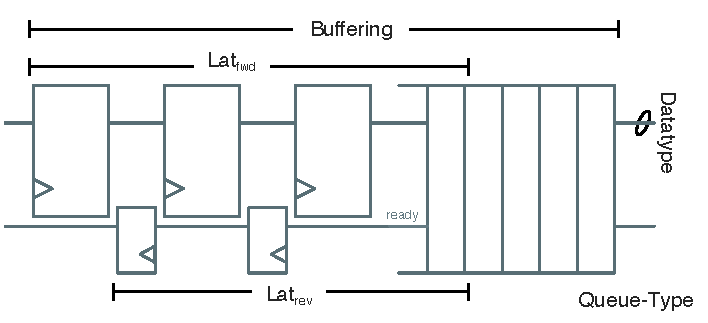
\includegraphics[width=\columnwidth]{figures/queue-channel.pdf}
        \caption{A queue type channel with its four characteristic parameters.}
        % graffle2pdf -c queue midas-graphics/graffle/channel-types.graffle figures/queue-channel.pdf
        \label{fig:queue-channel}
    \end{subfigure}
    \begin{subfigure}[t]{0.34\textwidth}
        \captionsetup{margin=0.25cm}
        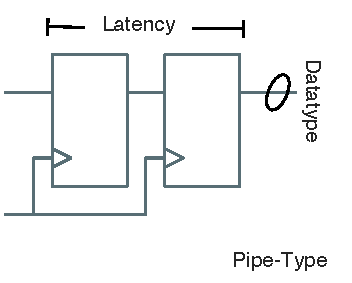
\includegraphics[width=\columnwidth]{figures/pipe-channel.pdf}
        \caption{A pipe-type channel. Setting latency to zero models a wire.}
        % graffle2pdf -c pipe midas-graphics/graffle/channel-types.graffle figures/pipe-channel.pdf
        \label{fig:pipe-channel}
    \end{subfigure}
    \centering
    \caption{Two types of channels used in a channel-bootstrapped formalism.}
\end{figure}


Addressing this, APort Networks~\cite{APortNetworks} was designed to support
finer-grained LPs that are coupled with register stages in the target. In their
paper, Pelleaur et al. use a processor pipeline as a motivating example and
divide different pipeline stages into seperate LPs. Later versions of the RAMP
architecture introduced the same sort of channel, which we call a \emph{pipe}
channel, shown in Figure~\ref{fig:pipe-channel}.  Pipe channels are defined by
a single parameter $l$, corresponding to their latency. Assuming the underlying
registers they model are not reset explicitly a using target signal, but are
instead initialized at time 0 to some statically known value, pipe channels
provide $l$ initial messages before they must stall for an input message.

Neither formalism appears to give any treatment to modeling a target-driven reset in
channels, as they both rely on time-zero intialization to effectively
"reset" target state.  We note that if these underlying state elements are
synchronously reset, the channels with $l >= 1$ may provide no more than 1
initial message, as future messages may causually depend on a reset
message\footnote{We further note that neither of these formalisms was designed
to support asynchronously reset as all-events are synchronous to an implicit
clock. At a first blush, however, asynchronous reset mandates that that even
the first message emitted by a pipe-channel with $l > 0$ would depend causually
on reset at time 0.}. A pipe-type channel with $l = 0$, is a degenerate LP that models a wire between the producer and consumer LP, coupling them combinationally.
It models no target state and merely relays messages from producer to consumer.

In both formalisms, units model a single target cycle of execution by dequeuing an input message
from each of its input ports, and enqueing a new output message into each of
it's output ports. The simplest unit implementation, and the one perscribed by
APort Networks, waits for all input messages to arrive and all of it's output
ports to be ready to accept to messages, before it may \emph{fire}. Then the
unit computes its state updates and simulateously enqueues a single output
message into each output port, and dequeues a message from each input port.
Figure~\ref{fig:adder-example} demonstrates the execution of a single target cycle in a channel-bootstrapped formalism.

\begin{figure}
    \centering
    \begin{subfigure}[t]{0.49\textwidth}
        \captionsetup{margin=0.25cm}
        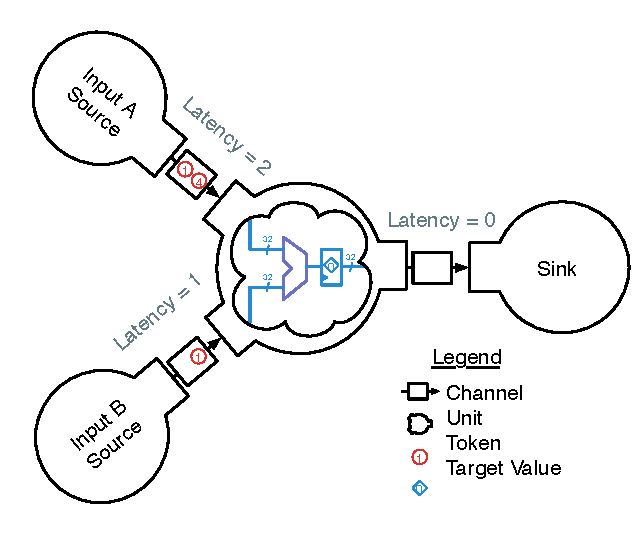
\includegraphics[width=\columnwidth]{figures/adder-example1.pdf}
        \caption{Initial state of the graph.}
        % graffle2pdf -c initial-state midas-graphics/graffle/adder-example.graffle figures/adder-example1.pdf
    \end{subfigure}
    \begin{subfigure}[t]{0.49\textwidth}
        \captionsetup{margin=0.25cm}
        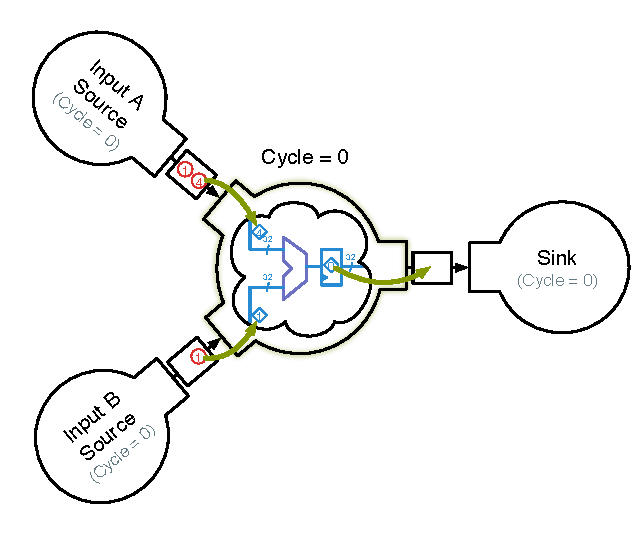
\includegraphics[width=\columnwidth]{figures/adder-example2.pdf}
        \caption{With all input tokens available, the unit fires and advances to cycle 1.}
        % graffle2pdf -c tfire-cycle0 midas-graphics/graffle/adder-example.graffle figures/adder-example2.pdf
    \end{subfigure}
    \begin{subfigure}[t]{0.49\textwidth}
        \captionsetup{margin=0.25cm}
        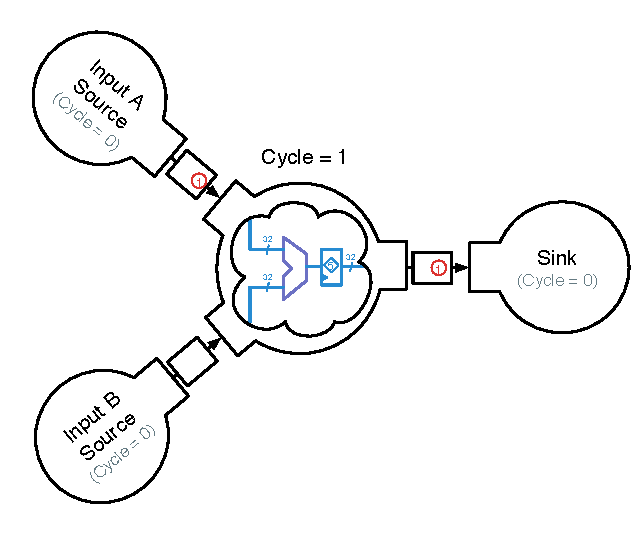
\includegraphics[width=\columnwidth]{figures/adder-example3.pdf}
        \caption{The state of the graph after firing. The unit is stalled on the arrival of a B-input token.}
        % graffle2pdf -c cycle1 midas-graphics/graffle/adder-example.graffle figures/adder-example3.pdf
    \end{subfigure}
    \begin{subfigure}[t]{0.49\textwidth}
        \captionsetup{margin=0.25cm}
        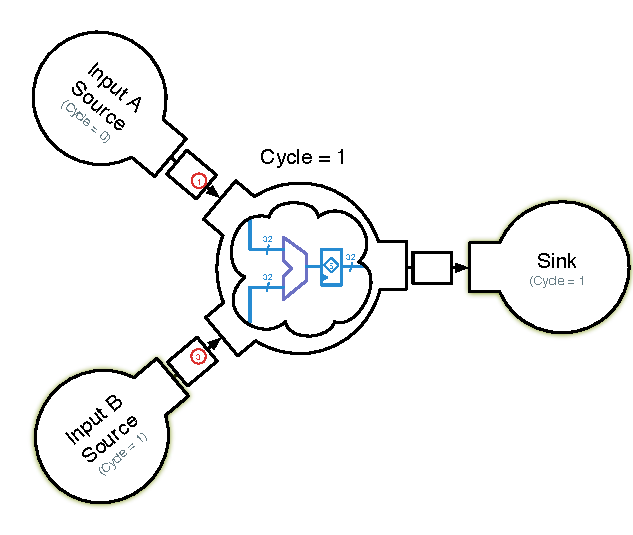
\includegraphics[width=\columnwidth]{figures/adder-example4.pdf}
        \caption{Input B source fires, producing the needed token.}
        % graffle2pdf -c inputb-fires midas-graphics/graffle/adder-example.graffle figures/adder-example4.pdf
    \end{subfigure}
    \begin{subfigure}[t]{0.49\textwidth}
        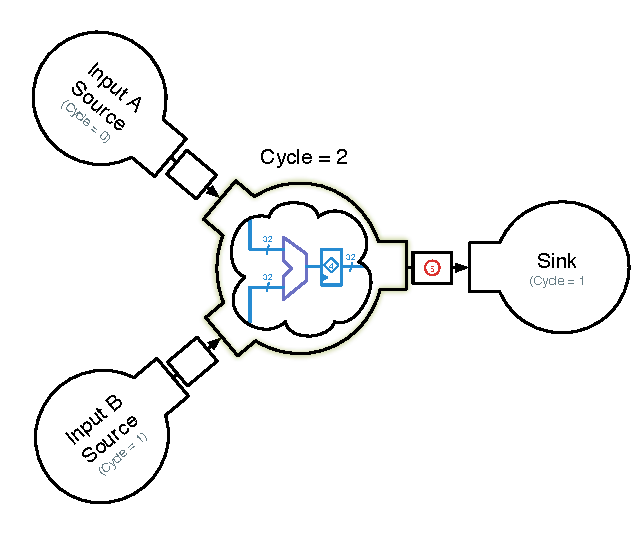
\includegraphics[width=\columnwidth]{figures/adder-example5.pdf}
        \caption{The state of the graph after two firings of the unit.}
        % graffle2pdf -c cycle2 midas-graphics/graffle/adder-example.graffle figures/adder-example5.pdf
    \end{subfigure}
    \centering
    \vspace{-0.25in}
    \caption{A 32-bit adder model and environment simulating a single cycle of target time.}
    \label{fig:adder-example}
\end{figure}

If the simulation designer uses exclusively, non-wire-type channels both
formalisms are free of deadlock, as there exists no unit whose output at cycle
$t$ depends on the output of another unit also at cycle $t$\footnote{From a
conservative PDES persective, every LP has a non-zero lookahead, and given that
every LP sends messages at every timestamp (obviating the need for null
messages), deadlock is avoided by construction}. In these simulators, all units
can excute cycle $t$ concurrently, which assuming no other sources of delay,
permits the simulator to run at unity FMR.  However, as with latency-insensitive boundaries, it is not always possible to define LP
at registered boundaries.  The use of wire-type channels, (i.e. combinational
coupling between LPs) that introduces two principle challenges: at best, it
increases simulator FMR, and at worst, it may introduce time-zero simulation
deadlock. To illustrate each of these effects, in Figure~\ref{fig:channel-deadlock} we consider a
latency-insensitive interface between two units implemented three different ways: with a queue-type
channel, with one pipe and one wire-type channel, and with two wire-type channels.

\begin{figure}
    \centering
    \begin{subfigure}[t]{0.49\textwidth}
        \captionsetup{margin=0.25cm}
        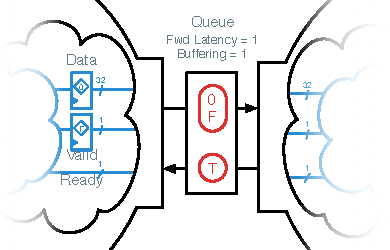
\includegraphics[width=\columnwidth]{figures/li-queue-channel-manual.pdf}
        \caption{A RAMP-style queue-type channel. This allows both models to
        fire simultaenously, but may only be used if it is acceptable to model
        a target queue in the channel.}
        %  -c queue midas-graphics/graffle/deadlock.graffle figures/li-queue-channel.pdf
    \end{subfigure}
    \begin{subfigure}[t]{0.49\textwidth}
        \captionsetup{margin=0.25cm}
        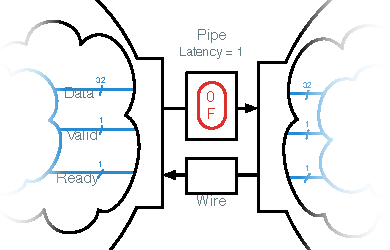
\includegraphics[width=\columnwidth]{figures/li-pipe-channel-manual.pdf}
        \caption{One pipe-type channel, and one-wire type channel carrying the backpressure. This leads $FMR >= 2$, with the consumer unit
        firing first to produce a backpressure token that is subsequently consumed by the producer unit.}
        %  -c pipe midas-graphics/graffle/deadlock.graffle figures/li-pipe-channel.pdf
    \end{subfigure}
    \begin{subfigure}[t]{0.49\textwidth}
        \captionsetup{margin=0.25cm}
        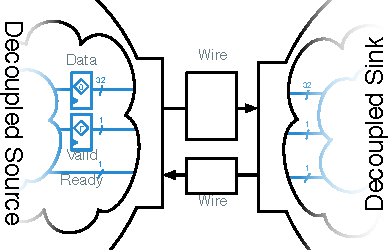
\includegraphics[width=\columnwidth]{figures/li-wire-channel-manual.pdf}
        \caption{Two-wire type channels. This deadlocks an APort Network, as neither producer nor consumer unit can fire
        before the other.}
        % -c wire midas-graphics/graffle/deadlock.graffle figures/li-wire-channel.pdf
    \end{subfigure}
    \centering
    \vspace{-0.25in}
    \caption{Three potential channel modelling decisions for a latency insensitive interface between two units.}
    \label{fig:channel-deadlock}
\end{figure}

In the absence of deadlock, wire-type channels tend to increase FMR as in
general a combinational path that spans $N$, units will take $N$ cycles to
execute. Note that other channels connecting these units tends to prevent
pipelining multiple cycles of target execution (i.e., this latency cannot be
overlapped, with the simulation of younger target cycles).

Deadlock is the more pressing challenge. Wire-type channels remove the
aforementioned property that all LPs have non-zero lookahead.  Here there are
two situations that may emerge. If the target itself has a combinational loop,
the behavior of the physical system is itself undefined, and simulation
deadlock is unavoidable~\footnote{We note it is possible to have "false"
combinational loops but many tools reject these patterns, and so it's not
unreasonable to ban them in these simulators as well.}. As a matter of
practise, hardware designers know to avoid combinational loops. The second
challenge arises from poor LP implementation, such as the unit perscribed by
APort Networks, that attempts to enqueue and dequeue multiple messages
atomically. Mandating this implementation has the effect of introducing a
dependency between all output messages on all input messages, even though there
they may be no combinational path between many of these outputs and inputs in
the underlying target. Given its definition of a unit, APort Networks do not
give the correct set of constraints to avoid deadlock as a graph that contains
a cycle of wire-type channels -- that do not represent a combinational loop in
the target -- deadlocks at time zero.


\subsection{Latency-Insensitive Bounded-Dataflow Networks}

Unlike channel bootstrapped formalisms, LI-BDNs avoid deadlock by imposing
different constraints on the implementation of LPs based on the underlying
hardware they model, and remove the need for specialized channels to bootstrap
simulation. Since connections between LPs always represent wire-like
connectivity, LI-BDNs impose no contraints on how the target
is divided into LPs. LI-BDNs were originally developed as a more flexible abstraction for building
latency-sensitive designs that preserve the RTL timing of a synchronous circuit, extending
the work of Carloni et al., in the Theory of Latency Insensitive Design, however the authors identify that this problem is analogous
to constructing an ITDC simulator from synchronous ASIC RTL.

In the terms of the paper, what we have loosely referred to as a synchronous
block of RTL thus far is defined synchronous sequential machine~(SSM). Vijayaraghavan et
al.\cite{LIBDN} formally define an SSM:

\begin{widequote}
An SSM is a network of combinational operators or gates
such as AND, OR, NOT, and state elements such as registers,
provided the network does not contain any cycles which has
only combinational elements.
\end{widequote}

Missing from this definition is any treatment of multiple clock domains, different
types of state elements, asynchronous set or reset.  Inherent to the name
``synchronous'', Vijayaraghavan et al. forbid their existence -- in an SSM
\emph{all} state updates occur simultaenously. While this limits the
applicability of their approach, much of a modern SoC, such as the islands of a
GALS-based design, locally meets this definition.  With it's simple
state-update semantics, any SSM can be easily converted into a \emph{patient}
SSM; the equivalent circuit whose state update can be controlled with the assertion of a global enable signal.
One way this conversion can be achieved, proposed by the authors, is by
disabling register updates and masking off RAM write-enables when this control
signal is unset. Alternatively, we note that the SSM may be clock gated.

With an SSM defined, we can now define an LI-BDN, and how they can be used to implement any
SSM in an latency-insensitive manner. An LI-BDN is a dataflow network of latency-insensitive nodes whose
edges represent FIFO communication channels with non-zero, but finite (hence,
bounded) capacity. The latency-insensitive nodes of the graph are
referred to as \emph{Primitive LI-BDNs}~(in PDES terms, these are LPs), which is to say, they 
are not themselves subgraphs of more than one node. A
LI-BDN is said to \emph{implement} an SSM, if it \emph{partially implements}
the SSM, and is deadlock free. In the terms of a hardware engineer, partial implementation~(PI) implies that
the message trace of outputs from the ports of the LI-BDN "matches" the
per-cycle trace of outputs from the SSM. Vijayaraghavan et al.\cite{LIBDN}
formally define PI:

\begin{widequote}
A BDN $R$ partially implements an SSM $S$ iff
\begin{enumerate}
\item There is a bijective mapping between the inputs of $S$ and
[the input tokens of] $R$, and a bijective mapping between the outputs of $S$ and
[the output tokens of] $R$.
\item The output histories of $S$ and $R$ match whenever the
input histories match, i.e.,
\begin{align*}
\forall n &> 0\\
&\text{$I(k)$ for $S$ and $R$ matches $(1 \leq k \leq n)$}\\
\Rightarrow &\text{$O(j)$ for $S$ and $R$ matches $(1 \leq j \leq n)$}
\end{align*}
\end{enumerate}
\end{widequote}

All SSMs have infinitely many possible partial implementations~\footnote{For
instance, one can take any existing partial implementation, and introduce an
extra cycle of delay on any of its outputs. As we'll show later, since it's
always possible to produce an LI-BDN from any SSM, it follows by induction that are infinitely many partial implementations
for any SSM.}, though some implementations deadlock when composed into larger graphs.
Consider the unit implementation perscribed by APort Networks. It is a valid partial implementation of
the source RTL, however, it cannot \emph{implement} a larger SSM when it is composed 
with other liked-styled implementations without the use of non-wire-type channels (which themselves
are a special form of LP that remove zero-cycle loops between units).
Conversly, LI-BDNs garauntee deadlock freedom by adhering to two additional properties.
The first is \emph{No Extraenous Depedencies}~(NED) which defines when an LP is obligated to enqueue output messages. Vijayaraghavan et al.\cite{LIBDN} formally define NED:

\begin{widequote}
A primitive BDN has the NED property if all output FIFOs have been enqueued at least $n-1$ times,
and for each output $O_i$, all the FIFOs for the inputs in $\emph{CombinationallyConnected}(O_i)$
are enqueued $n$ times, and all other input FIFOs are enqueued at least $n-1$ times, then $O_i$ FIFO
must eventually be enqueued $n$ times.
\end{widequote}\label{def:ned}

One intuitive explanation of NED is that it exploits the same observation that
permits a pipe-type channel to send output messages before receiving any input
messages: any output driven only by state in the LP (i.e., outputs not
combinationally coupled to an input) can enqueue an output messages for cycle
$t$ before receiving any input messages for cycle $t$. NED broadens this to apply to logic cones fed not just by state
elements but those that depend only on a subset of the LP's inputs.

The second property an LI-BDN must satisfy is the \emph{self-cleaning}~(SC) property. SC 
defines when an LP is obligated to dequeue input tokens. Vijayaraghavan et al.\cite{LIBDN} formally define SC:

\begin{widequote}
A primitive BDN has the SC property, if when all the
outputs are enqueued $n$ times, all the input FIFOs must
[eventually]\footnote{Clarified in~\cite{LIBDNMasters}.} be dequeued $n$ times, assuming an infinite source for each
input.
\end{widequote}\label{def:sc}

While the nodes of an APort Network do not always satisfy NED, they do satisfy
SC. At it's heart, SC provides an assurance that LPs drain their input FIFOs,
allowing those FIFOs remain bounded. We note that if an LP fails to satisfy
SC, it will likely fail to partially implement its SSM unless its outputs are
completely independent of the inputs from which it is failing to dequeue. In
this case having unbounded FIFOs would suffice to prevent deadlock.

Of particular concern to this dissertation is a method through which an SSM can
be converted into a primitive LI-BDN.  Vijayaraghavan et al. describe a means that uses
a wrapper module around the patient SSM based on it's combinational
depedencies. The SSM is treated as a black box otherwise. The wrapper circuit,
for a single output, is shown in \ref{figure}. This method is highly amenable
to automation with a FAME compiler, as it requires only the ability analyze
combinational depedencies in the underlying SSM.

\section{The MIDAS Compiler \& Simulator Microarchitecture}

As we first introduce in Section~\ref{sec:midas-intro} mentioned previously,
MIDAS was our first attempt at building a RAMP compiler. Here we describe the
version of MIDAS released with FireSim 1.5.0, which differs modestly from earlier iterations 
described in the CARRV paper~\cite{MIDAS} and Donggyu Kim's dissertation~\cite{DGKDissertation}.

MIDAS generates ITDC simulators directly from ASIC RTL; these simulators that
implement a channel-bootstrapped formalism, with all target graphs having a
star topology. We show an example graph for a Rocket-Chip-based system, the
most commonly used target generator in MIDAS, in Figure~\ref{fig:rocket-target-graph}
"hub" unit is transformed from ASIC RTL elaborated by a user-provided Chisel
generator. This RTL does not represent a
closed system -- it exposes I/O interfaces that must be tied to units that model those
devices. These units are called \emph{endpoints} and form satelite nodes in the graph.
MIDAS-generated simulators are designed to run on hybrid CPU-FPGA hosts
with the expectation being that certain tightly coupled endpoints, such a DRAM
timing models, will be written in RTL and hosted on the FPGA, while other higher
latency, less performance critical ones, such UART and block device models, can
be written in software hosted on the CPU. We refer to the CPU-hosted componenet
of the simulator as the \emph{driver}. To avoid deadlock and provide good
simulation FMR, MIDAS injects queue-type channels (to model a 2-deep,
fully-decoupled FIFO) on all decoupled interfaces, and 1-cycle-latency
pipe-type channels. Assuming units do not stall internally, MIDAS-generated
simulators can run at unity FMR. We show an example simulator mapped to an EC2 F1 host in Figure~\ref{fig:mapped-simulator-f1}.

\begin{figure}
    \centering
    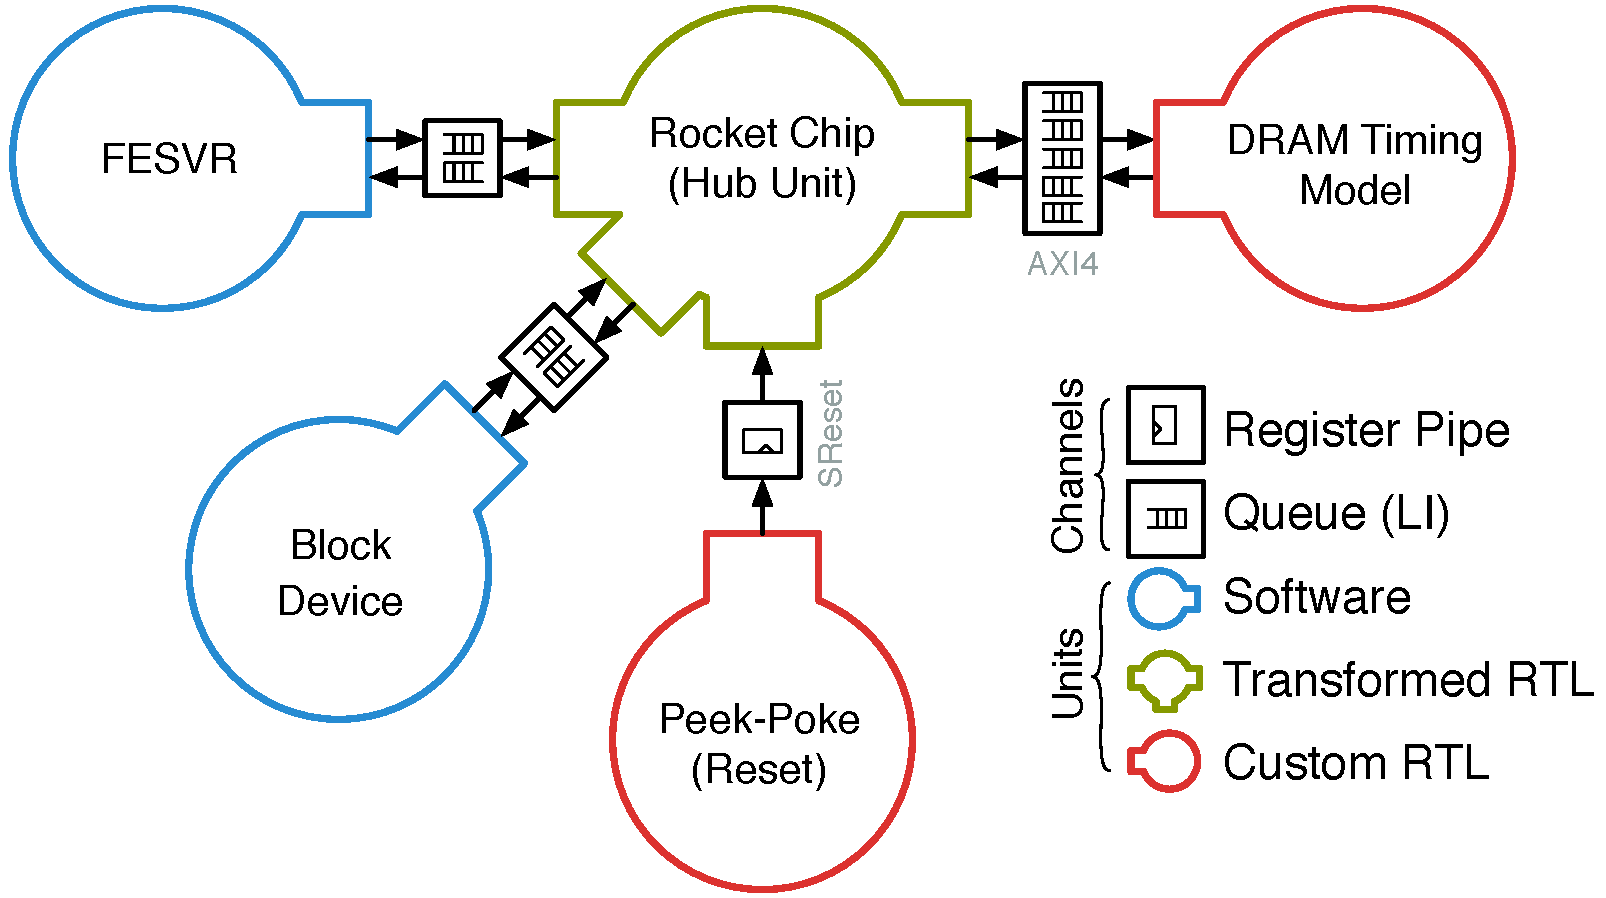
\includegraphics[width=0.9\textwidth]{figures/rocket-target-graph.pdf}
    % graffle2pdf -c rocket-target-graph midas-graphics/graffle/masters-target.graffle figures/rocket-target-graph.pdf
    \caption{The graph of a typical Rocket-Chip-derived system.}
    \label{fig:rocket-target-graph}
\end{figure}

\begin{figure}
    \centering
    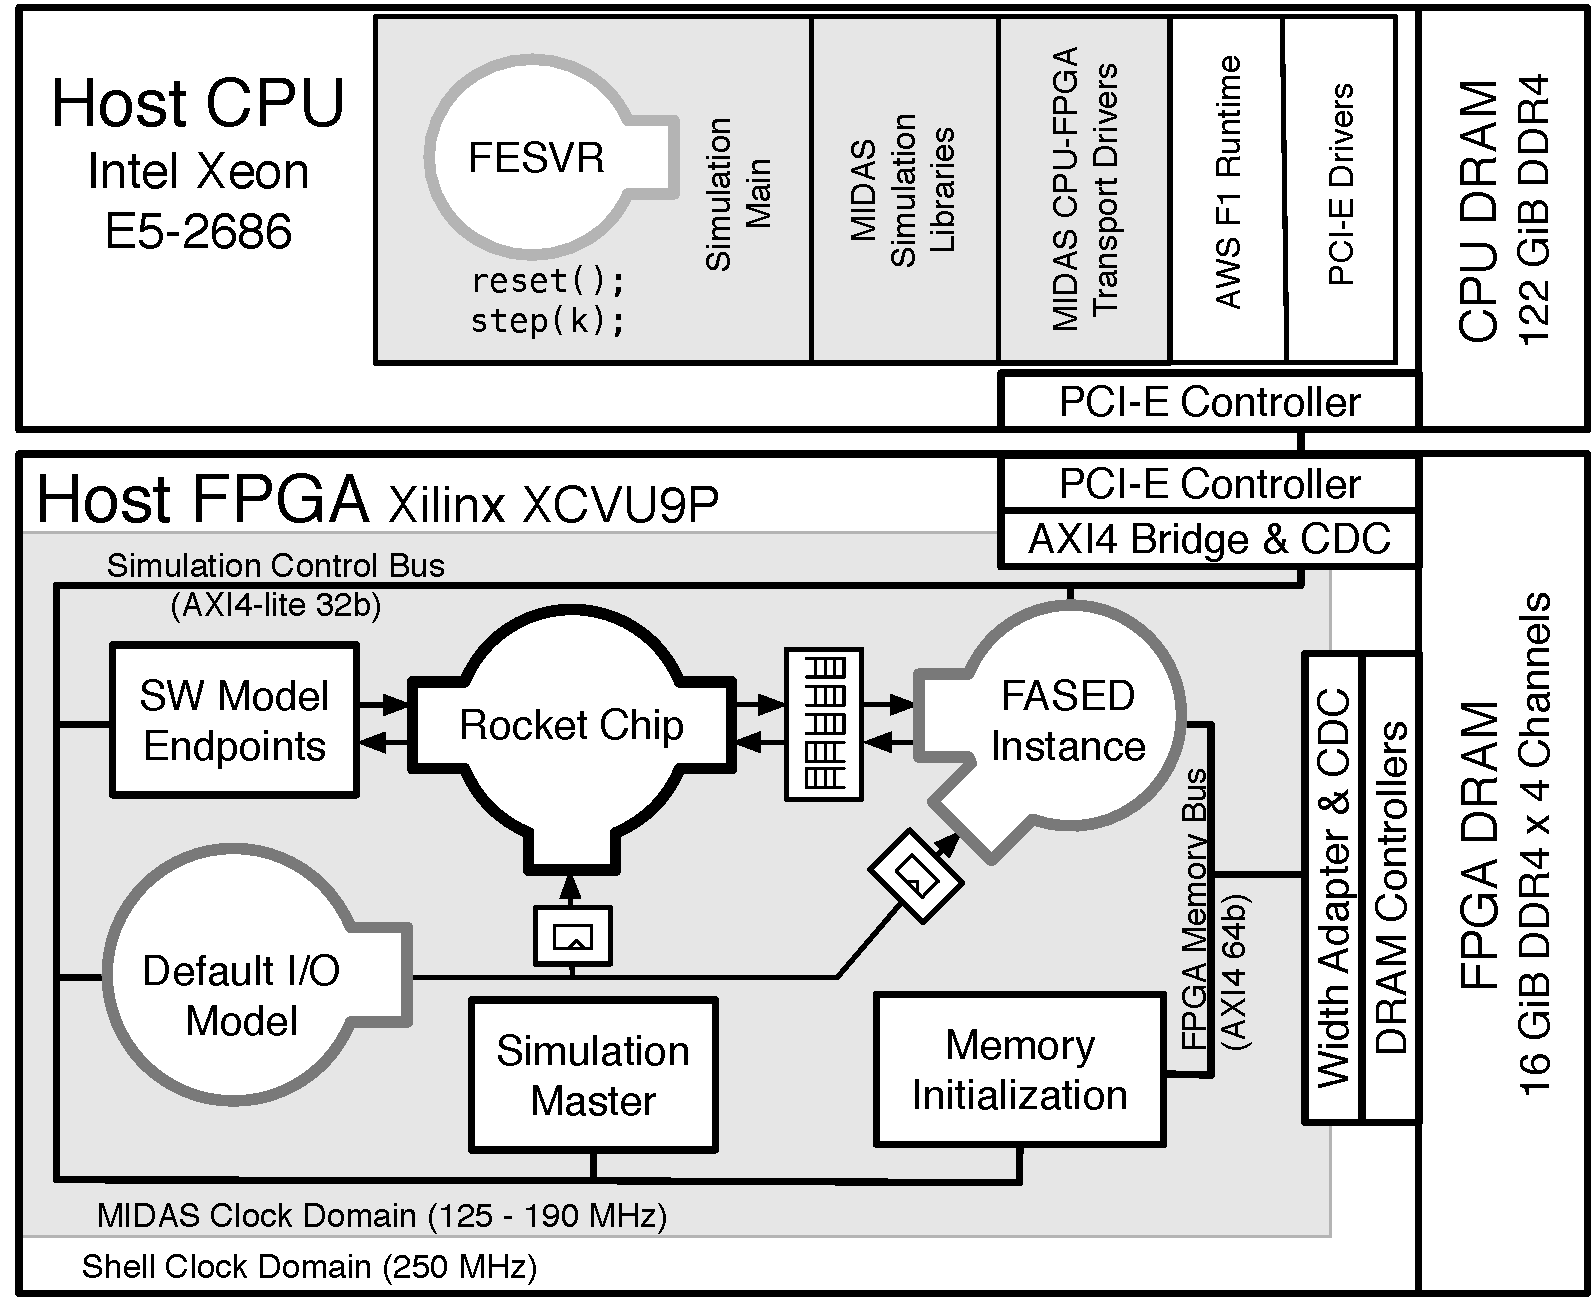
\includegraphics[width=0.9\textwidth]{figures/mapped-simulator-f1.pdf}
    % graffle2pdf -c f1 midas-graphics/graffle/mapped-simulator.graffle figures/mapped-simulator-f1.pdf
    \caption{An example simulator mapped to and EC2 F1 host.}
    \label{fig:mapped-simulator-f1}
\end{figure}


\subsection{Endpoint Units}

Topological position aside, endpoint units differ from the hub in that they are not transformed from ASIC
RTL and instead are written by hand, and thus, not exact models of the desired target system.
Endpoints consist of an \emph{endpoint module}, which resides on the FPGA and drives the channels bound to the hub unit, and an
\emph{endpoint driver}, which is linked into the main simulation driver and hosted on a CPU.
Even the purest "CPU-hosted" units require an endpoint driver that
implements transport for token streams moving on and off the
FPGA\footnote{FireSim stitched together larger targets by adding software units
to represent parts of the network. These were hosted purely on a CPU, often
with no FPGA attached.} Similarly, FPGA-hosted models tend to have a driver
that is reponsible for configuring the FPGA-hosted piece of the unit, and for
polling FPGA-hosted instrumentation.

Endpoints can leverage three types of host resources:

\begin{enumerate}
\item CPU-mastered MMIO. Here, modules expose 32-bit registers that can be
    written to and read from the driver. This is typically used to expose
    configuration  parameters that the driver initializes before simulation
    commences, and to expose instrumentation that can be polled during
    simulation. Generally, MMIO cannot provide enough bandwidth to support transporting token streams,
    for low-bandwidth, loosely coupled endpoint it can also be used to pass transaction-level messages.
    The endpoints for UART and the FireSim block device do this.

\item CPU-mastered DMA. To support moving complete token streams, endpoints can
    bind to CPU-mastered DMA. Here endpoint modules expose hardware FIFOs to the DMA bus to which the driver
    can make bulk (up to 4192KB) reads and writes. If the endpoint is not closely coupled
    to the hub, token transport can be overlapped with simulator execution: the NIC endpoint relies on this
    provide good FMR in networked simulations~\cite{FireSim}. CPU-mastered DMA is also used 
    to drain token streams from instrumentation endpoints. Since these endpoints do not drive
    tokens back to the hub, it is only necessary to provide sufficient DMA read-bandwidth to achieve good FMR.
    Examples of this include the synthesized printf endpoint and the TracerV
    RISC-V instruction trace collection endpoint.

\item FPGA DRAM. Some units require more local storage than FPGA fabric can
    provide, but cannot afford the round trip latency of using CPU memory or
    disk. MIDAS provides a simple means to let endpoints drive the FPGA
    DRAM memory system.  MIDAS's memory timing models, both those described
    in the CARRV publication~\cite{Midas} and later by FASED~\cite{FASED},
    use FPGA DRAM as a backing store for a timing model that's implemented
    in FPGA fabric.
\end{enumerate}

Endpoint drivers interact with their associated module using four methods
exposed by the main simulation driver: \texttt{simif::read} and
\text{simif::write} drive CPU-mastered MMIO; \texttt{simif::pull} and
\texttt{simif::push} are used to drive CPU-mastered DMA.

\subsection{Simulation Driver}

The simulation driver is written in C++ and instantiates an endpoint driver class for each endpoint
in the system. Once the FPGA has been flashed, the driver can be launched.
Simulation proceeds in three phases:

\begin{enumerate}
    \item Initialization. This provides a window for endpoint drivers to do DMA
        and MMIO before the simulation commences.  Here the driver optionally
        zeros-out or intializes FPGA DRAM, before calling each endpoint
        driver's \texttt{init} method, which sets up configuration registers on
        the FPGA that may control timing parameters or instrumentation modes.

    \item Execution. Here the driver invokes each endpoint's \texttt{tick}
        method in a tight loop, in round-robin order.  Drivers issue MMIO and
        DMA requests attempting to make forward progress without blocking.

    \item Teardown. Simulation ends once any endpoint driver calls for
        termination. The driver calls each endpoint's \texttt{finish} method,
        which gives the endpoint a final opportunity to do FPGA DMA and MMIO. This
        typically includes reading final FPGA-hosted intrumentation values and commiting simulation output to disk.
\end{enumerate}


\subsection{Time Control}
After FPGA programming and reset, channels are ready to produce initial tokens and thus units are free
to begin executing. Generally, endpoints that require
configuration wait for an MMIO register to be set during the driver's
intialization phase before acting on token streams. In the absence of
user-provided endpoints, MIDAS prevents the hub model from free-running by
mandating that all target designs have a synchronous reset that is driven
by a special \emph{peek-poke} endpoint. The peek-poke endpoint ties off all
unnconnected I/O on the target to memory-mapped registers
that can be driven to specific constants during initialization, or
periodically changed during simulation. The driver can then "step" the hub
by controlling the emission of reset tokens by the peek-poke endpoint.
Unlike for other endpoints, channels between the peek-poke endpoint and hub
are the only channels that are wire-type by default: enqueuing a $k$ reset
tokens permits the hub to advance no further than cycle $k$.

During simulation teardown, the simulator estimates the number of cycles simulated by
reporting the number of reset tokens enqueued by the endpoint. In practise,
the hub may not have drained all tokens in the reset channel (it is in the
past relative to the peek-poke endpoint), and additionally, other endpoints
connected to the hub may be relatively more or less advanced in simulation
time due to the distributed nature of the simulator.

\subsection{Using MIDAS: Generator Side Integration}

MIDAS functions by providing an alternate generation flow for a chisel
generator.  In their Scala application, the user lazily instantiates their
module class and calls out to chisel elaboration as they normally would.
This produces a FIRRTL circuit and annotations for what will become the hub
model.  Typically the lifetime of a chisel module class ends after
elaboration, however the lazy reference to the class allows the user to
extract the Scala types and names of the I/O interfaces of the top-level
module after elaboration. This is critical as MIDAS determines how to bind
endpoints to the hub unit by querying a user-provided map of Chisel type to
endpoint module for each of the extracted I/O interfaces. Finally, the user
invokes the compiler, passing the FIRRTL circuit and annotations, the
extracted I/O list, separate lists of FIRRTL transforms to run on the
elaborated RTL and then the complete simulator, and an implicit parameters
instance which provides the aforementioned map and set switches to control
various stages of the compiler.

\subsection{MIDAS Compiler Flow}

\begin{figure}
    \centering
    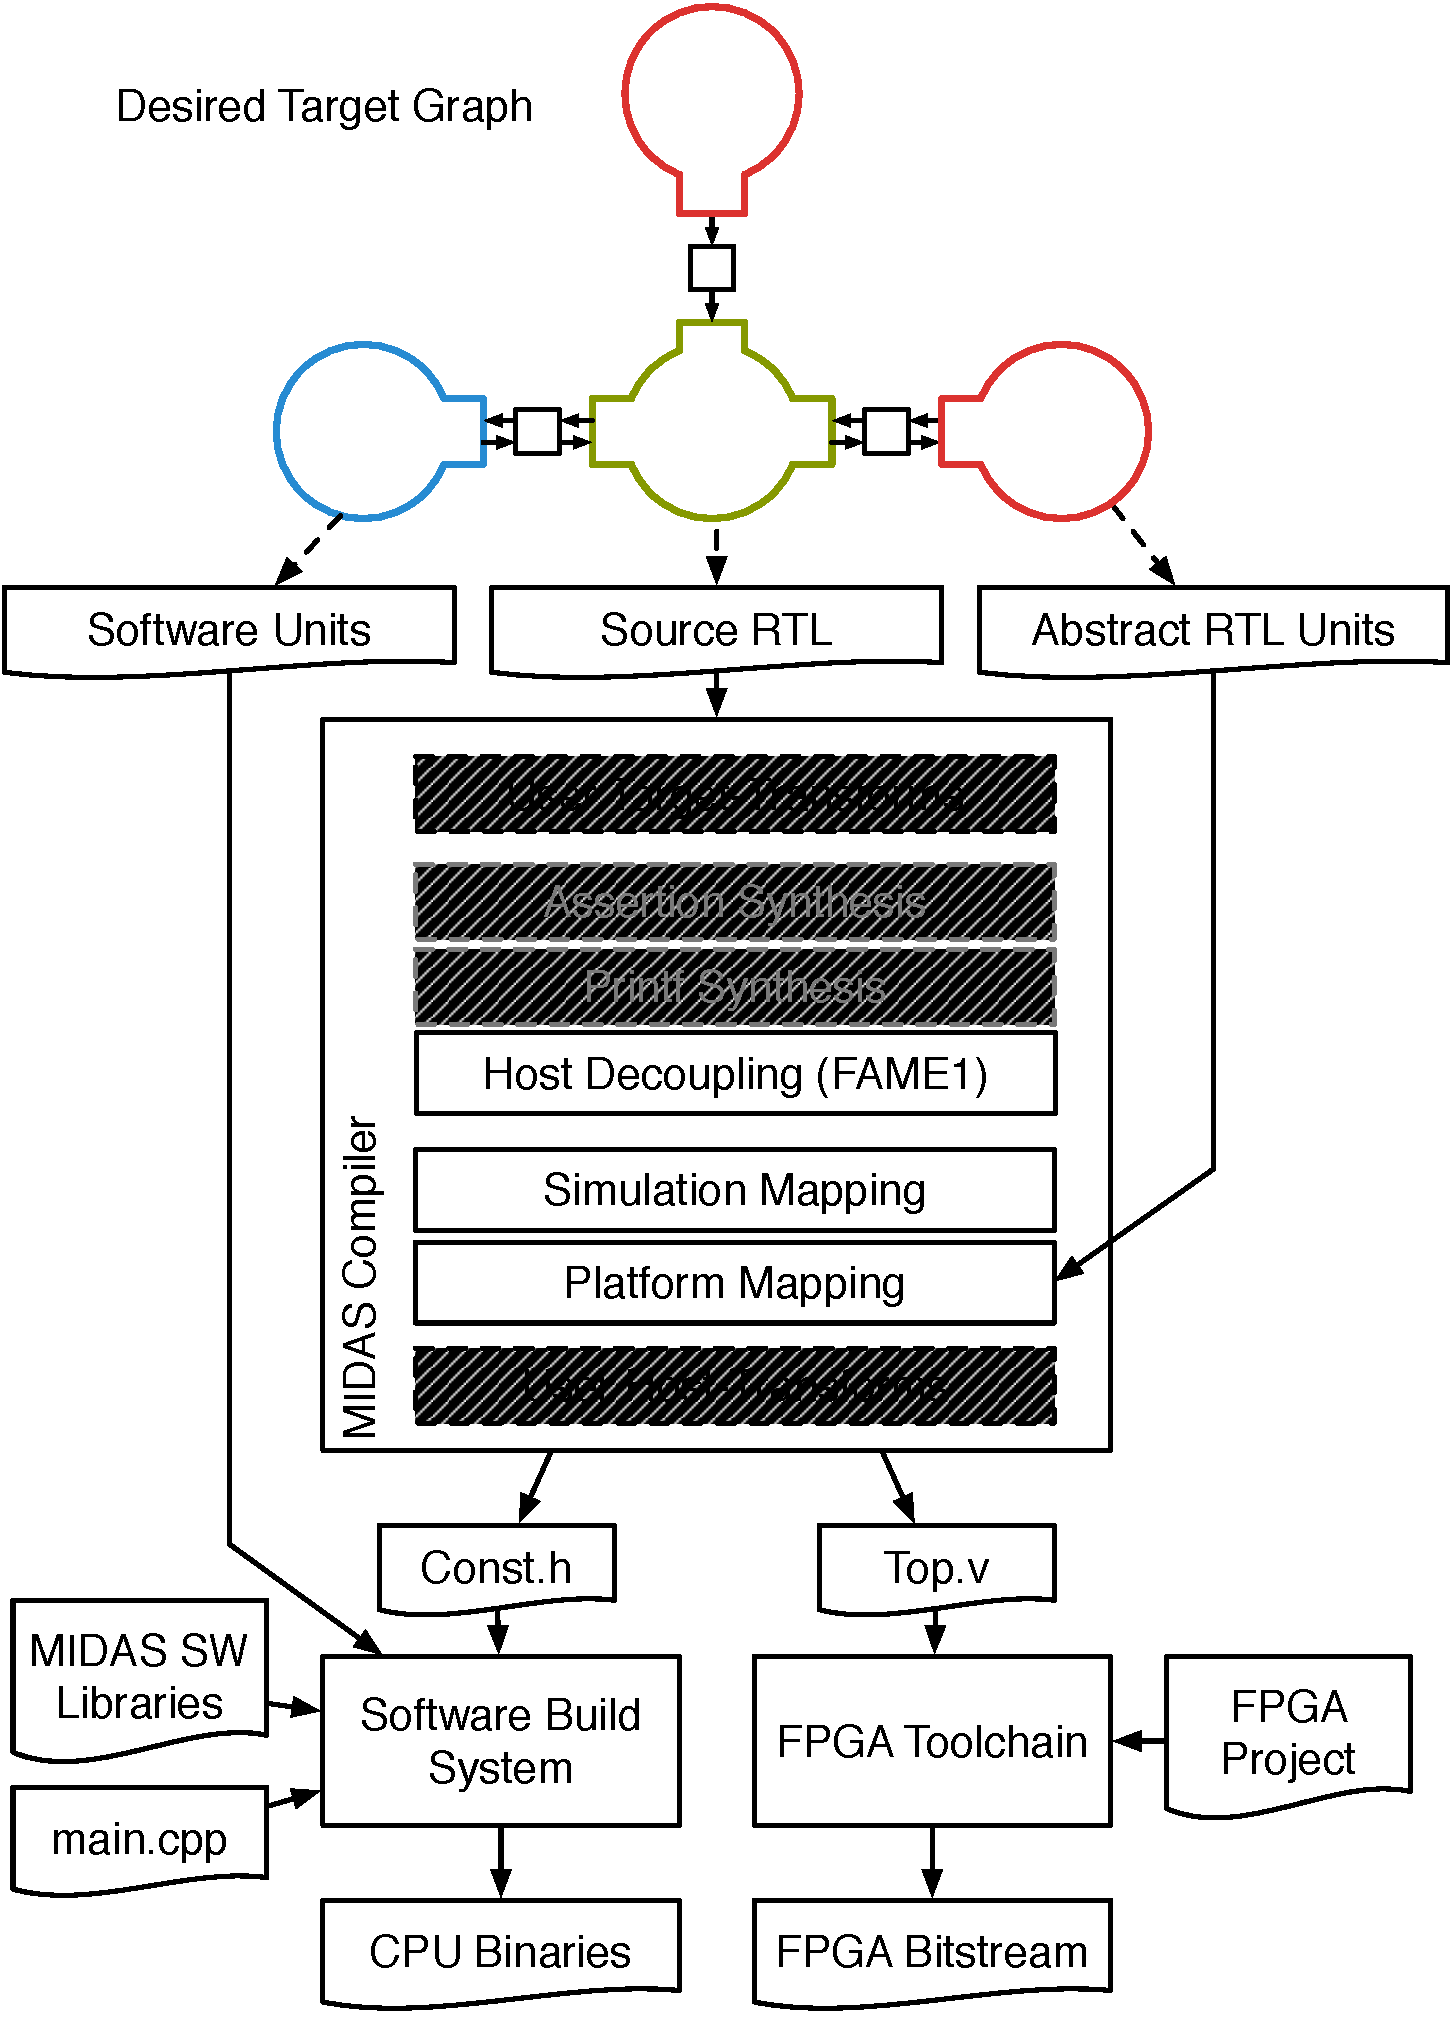
\includegraphics[width=0.9\textwidth]{figures/midas-flow.pdf}
    % graffle2pdf -c midas-flow midas-graphics/graffle/toolchain.graffle figures/midas-flow.pdf
    \caption{The end-to-end flow of a MIDAS compilation.}
    \label{fig:midas-flow}
\end{figure}

    We show the flow the MIDAS compiler in Figure~\ref{fig:midas-flow}.

    Before running core transformations, MIDAS schedules user-provided target transforms.
    In FireSim, dedicated passes to remove unsupported verilog black-boxes and
    replace asynchronously reset registers synchronously reset ones.

    Next MIDAS runs instrumentation transformations, including printf synthesis
    and assertion synthesis~(these were initially presented in DESSERT~\cite{DESSERT}), if they have been requested by the user. These
    transformations "synthesize" \texttt{printf} and \texttt{stop} FIRRTL IR
    nodes by replacing them with a connections to new top-level outputs. Stops are
    replaced with a boolean that is asserted on cycles the stop condition is asserted. Similarly, printfs are replaced with an aggregate that contains
    the arguments for the printf's format string and an enable indicating the
    printf would trigger on that cycle. Like the other I/O interfaces, these new outputs will be bound to a single asssertion
    and printf endpoint later in the compiler.

    Now MIDAS runs its FAME-1 transform, transforming the RTL (an SSM) into a
    unit.  MIDAS converts the SSM into a patient SSM by injecting clock-enables
    on all registers (this introduces a 2:1 mux on register inputs) and by
    masking FIRRTL memory write enables. The transform divides and maps the
    SSM's I/Os into message ports by recursing through their corresponding Chisel types.
    Decoupled interfaces~(latency-insensitivity interfaces that use a ready-valid
    handshake) are split into a forward and reverse port, all other
    interface types are given a seperate port per leaf-element.  With the I/Os
    mapped into unit ports, the transform drives \texttt{fire} with the
    conjuction of all inputs' valid and all outputs ports' ready. The resulting
    unit is a direct implementation of an APort Network node.

    To complete the simulator, MIDAS then wraps the hub unit with two layers of Chisel-generated modules.
    In \emph{Simulation Mapping}, MIDAS again recursively walks the chisel-types of the I/O, this time
    to generate the channel implementations.
    Wire and pipe-type channels are implemented using a queue whose
    payload is the underlying hardware type of the target interface. The endpoint and hub can decouple
    as many cycles as these queues are deep.  Queue-type channels use a more sophisticated implementation
    that drives forward and reverse token streams. The queue channel
    implementation allows endpoint and hub to decouple under more specific runtime conditions~(for example,
    while a queue is not full it can continue to accept forward tokens and produce reverse tokens on its the producer side
    of the queue.

    In \emph{Host Platform Mapping}, MIDAS recursively walks the chisel-types
    of the I/O a final time, here it attempts to find a provided endpiont for
    each type using the Endpoint Map. If the map is defined on that type, MIDAS
    instantiates the endpoint module, and connects its tokenized host port to the freshly
    generated channels. All remaining unbound interfaces are then bound to the
    peek poke endpoint. Once all endpoints have been elaborated, it binds their
    MMIO interfaces and DMA interfaces, if present, to the simulation control
    and DMA buses, respectively, using a $1:N$ AXI4 arbiter. Memory timing
    models have their host-memory interface driven to DRAM memory interfaces,
    this time through an $M+1:N$ AXI4 crossbar, where $M$ is the number of
    target memory models and $N$ is the number of host memory channels. The
    extra master port is driven by the loadmem unit, which bridges the
    simulation control bus and memory bus and gives the driver the means to
    read and write to FPGA DRAM. The parameters of the host platform,
    specifically the width of these buses, and the number of memory channels
    are defined in the user-provided parameters instance. At this point MIDAS,
    generates a C++ header with all of the driver-required metadata for the
    simulator. Each endpoint module emits a fragment which contains its allocated MMIO and
    DMA addresses, as well as additional constructor parameters required by its
    endpoint driver.

    In a final step before verilog emission, MIDAS schedules the user's
    \emph{host transforms}.  This permits modifying the simulator RTL to futher
    customize it for a host platform. In FireSim, the \texttt{AutoILA}
    transform is run here to plumb out annotated signals to a Xilinx Integrated
    Logic Analyzer (ILA), which is required in for EC2 F1 hosts due to
    restrictions in Amazon's compilation flow. Finally, the FIRRTL optimization passes are run
    and the simulator verilog is emitted, and the compiler terminates.

    At this point, the users links the generated header into the simulation
    main, and compiles the generated verilog into a FPGA shell project.
    FireSim's build system automates much of this, and provides an FPGA shell
    project for EC2 F1 FPGAs. FireSim's manager \texttt{buildafi} will batch
    out bitstream builds to remote hosts on EC2. Similary, its
    \texttt{infrasetup} process compiles the simulation driver, in addition to
    preforming the other required tasks to prepare for running a simulation
    including flashing the an FPGA.

\section{Reviewing MIDAS's Limitations}

    At the end of the previous chapter, we indentified two limitations with MIDAS 
    that we aimed to address in Golden Gate. The first was that it did little to optimize
    FPGA resource utilization, precluding the its use for systems of non-trivial scale. 
    We considered a few possibilities: leaning on the endpoint system and user modifications to the target RTL,
    specialized transformations to implement specific optimizations as modifications to the hub model. What was clear to us
    is that we had a few objectives.

    - Minimize user modification to the ASIC RTL timing
    - Make it possible to optimize blocks that may be combinationally coupled to some part of the hub.
    - Provide rigorous mechanism verify the resulting simulator


    Ultimately, it was clear that the next compiler needed a generalized
    mechanism to identify and perform optimizations. To make it easier to
    implement optimizations, Golden Gate uses the LI-BDN target formalism,
    removing the explicit need for channels. We acknowledge that forcing
    optimizations to apply only at registered boundaries between units -- a
    requirement of a channel-bootstrapped formalism -- would produce simulators
    with better FMR, this would add complexity to passes in the compiler and
    might make some optimizations infesible.  We also note that these sorts of
    optimizations not fundamentally precluded by LI-BDN: when an edge between
    two LPs is driven by an output port with no combinational dependency on an
    input, it may be possible to implement that edge using flow queue to save a
    cycle of transmission latency.

    Moving to an LI-BDN formalism resolves a number of other modeling
    challenges MIDAS users face.  Requiring that non-wire-channels be injected
    between endpoints and the hub unit was too restrictive in some cases where
    the user wishes to model a combinational path that propagated through the
    endpoint. Another challenge was defining the reset semantics of these
    stateful channels.  MIDAS relies on FPGA programming to properly initialize
    these channels, however they are not held in \emph{target-reset} during
    simulation: it is purely coincidental that the hub model does not
    spuriously enqueue target data into queue-type channels while parts of the
    hub are under target reset. For a time, MIDAS would broadcast target reset
    tokens to channels and endpoints, but too is fraught as resets driving
    registers in the hub maybe different from this special-cased global reset.
    Instead of requiring that user specify this reset for each channel, LI-BDN
    can sidestep these issues entire by removing the need for stateful
    channels, allowing the compiler to assume fewer things about target.

    Supporting realistic simulations of systems with multiple clock domains,
    and asynchronous reset will take yet another rethinking as the
    SSM-assumption fundamental to LI-BDN and APort Network formalisms no longer
    applies. Here we introduce explicit timestamping into a sub-graph of
    simulator, and rely on a hardware implementation of the Chandy-Misra-Bryant
    algorithm using null-messages to avoid deadlock.  This explicitly timekept
    portion of the graph can co-exist with SSM optimizations which can be
    applied locally to parts of the design where the SSM assumption holds.



\chapter{Golden Gate: An Optimizing FAME Compiler}\label{sec:golden-gate}

\chapter{Stretching the Synchronous Assumption: Support for Systems with Rationally Related Clocks}\label{sec:static-multiclock}

\chapter{Embracing Asynchrony: Generalized Support For Asychronous Events via Explicit Timestamping}\label{sec:dynamic-multiclock}

%While \PNAME can compose with other FPGA-accelerated simulators, in this paper
we extend FireSim~\cite{firesim} and {\SIMNAME}~\cite{midas}. \SIMNAME is a
compiler that generates FPGA-accelerated simulators automatically from Chisel
RTL. MIDAS is not standalone; FireSim provides a development
environment, with RTL and software models for complete target designs, as well
and powerful utilities to batch out FPGA builds and simulations across Amazon EC2.

\section{Host-Target Decoupling}\label{sec:target-decoupling}
Generally, host-target decoupling begins with a \emph{target abstraction} that
represents the target and its environment as a dataflow graph of actors~\cite{LIBDN,APortNetworks}.  The target abstraction we use in this paper
derives from the one used in RAMP~\cite{RAMP} and resembles a
synchronous-dataflow graph~\cite{SDF} where:

\begin{itemize}
    \item \emph{Tokens} are messages passed between the nodes of the graph. Tokens represent
        the values on wires in the target at the end of a target cycle.
    \item \emph{Models} are graph nodes that model the behavior of a
        synchronous block of RTL. Each model executes one target cycle of
        simulation by dequeuing a token from each of its inputs and enqueuing
        a token into each of its outputs.
    \item \emph{Channels} are the edges of graph. They transport tokens
        between models and simulate target-interconnect latency, buffering, and clock-domain crossings. At the start of simulation, a channel is initialized with
        a number of tokens equal to its latency.
\end{itemize}
%
%\begin{figure*}
%	\centering
%    \begin{subfigure}[t]{0.32\textwidth}
%        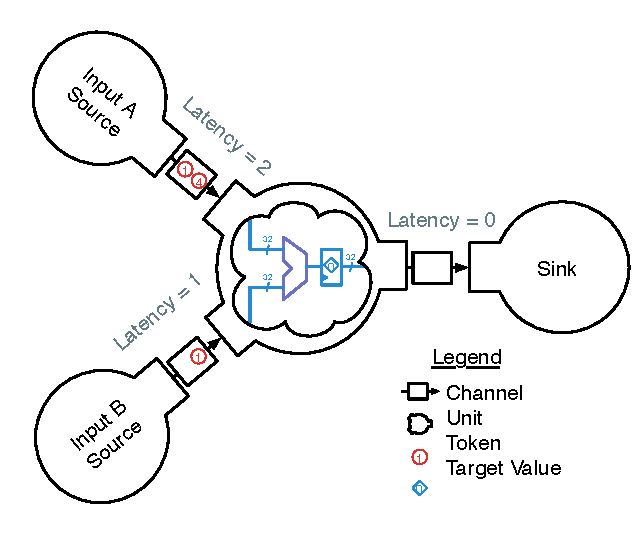
\includegraphics[width=\columnwidth]{figures/adder-example1.pdf}
%        % graffle3pdf -c initial-state midas-graphics/graffle/adder-example.graffle figures/adder-example1.pdf
%    \end{subfigure}
%    \begin{subfigure}[t]{0.32\textwidth}
%        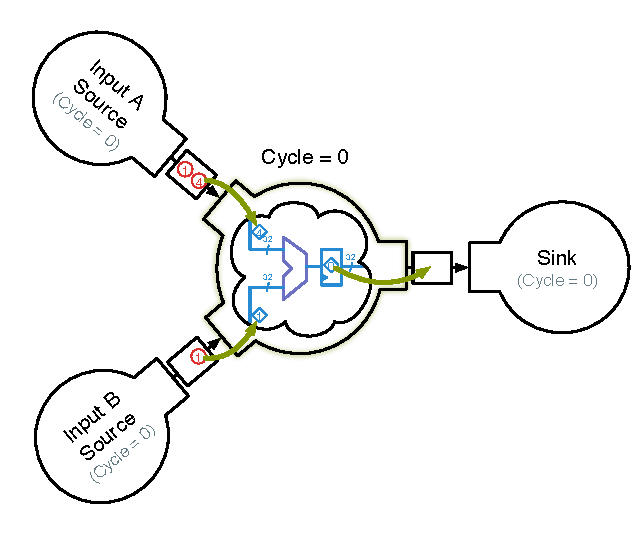
\includegraphics[width=\columnwidth]{figures/adder-example2.pdf}
%        % graffle3pdf -c tfire-cycle0 midas-graphics/graffle/adder-example.graffle figures/adder-example2.pdf
%    \end{subfigure}
%    \begin{subfigure}[t]{0.32\textwidth}
%        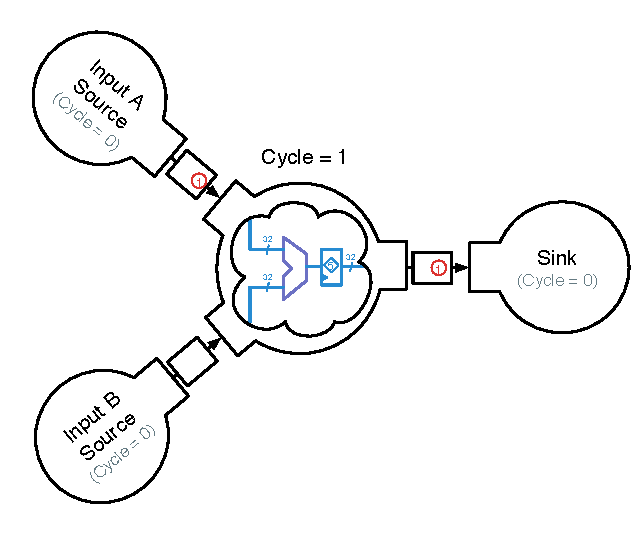
\includegraphics[width=\columnwidth]{figures/adder-example3.pdf}
%        % graffle3pdf -c cycle-1 midas-graphics/graffle/adder-example.graffle figures/adder-example3.pdf
%    \end{subfigure}
%	\centering
%    \caption{A 32-bit adder and environment simulating a single cycle of target time.}
%    \label{fig:adder-example}
%\vspace{-0.1in}
%\end{figure*}
%
%Figure~\ref{fig:adder-example} illustrates an example graph, consisting of a
%single 32-bit adder unit, composed with source and sink units, as it executes
%one cycle of target time.

A simulator that faithfully implements this graph decouples target time from
host time. Unlike in an FPGA prototype, where every FPGA clock cycle emulates a
target clock cycle, an FPGA-hosted model only executes a target-clock-cycle when
it can legally fire. Thus, the behavior of the target is decoupled from the
host, allowing simulators to be partitioned across the host and to tolerate
variable-host-latencies to DRAM and the CPU, while remaining deterministic.
Unfortunately, this results in target time advancing slower than it would in an
FPGA prototype of the same host frequency.  This is quantified by the
FPGA-cycle-to-Model-cycle Ratio~(FMR)\cite{APortNetworks}, below, which increases from
one~(the simulator simulates a target cycle on every FPGA host cycle) as the simulator stalls on token availability and backpressure. The FMR
of a simulator is variable: it is a function of both application-dependent
behavior in the target and variable latencies in host services.
$$ FMR = \frac{Cycles_{FPGA}}{Cycles_{Target}}$$

\section{The \SIMNAME Compilation Flow}\label{sec:fame1}
\SIMNAME-generated simulators compose three types of models in their target graphs:
\begin{enumerate}
    \item \emph{Transformed RTL} models generated from ASIC RTL.
    \item \emph{Abstract RTL} models intended for FPGA hosts.
    \item \emph{Software} models that are hosted on a CPU.
\end{enumerate}

The next three sections give an overview of how \SIMNAME, with the help of the
user, maps a target graph composed of these models into an FPGA-accelerated
simulator.

\subsection{ASIC-RTL-to-Model Transformation}\label{sec:fame1}
We transform a synchronous block of RTL into a model using a FIRRTL~\cite{firrtl} transformation called a \emph{FAME-1}
transform. The transformation gates state update of the RTL with a model-global
signal, \emph{targetFire}, which is driven with the AND-reduction of the valid
signals of all input ports and the ready signals of all output ports.  Thus, in
these models, state update, output token enqueue, and input token dequeue occur
simultaneously in a single host-clock-cycle.

\subsection{FPGA-Host Mapping}

Once ASIC-RTL has been transformed into models, \SIMNAME creates a host-agnostic
mapping of the target graph. This is also the point where \SIMNAME links in
other models, including \PNAME instances.

Using Chisel, \SIMNAME generates simulation FIFOs that implement the channels of
the target graph.  When a channel spans the boundary of the FPGA, \SIMNAME
generates an \emph{endpoint}, a FIFO with a matching head or tail on the
opposite part of the host platform.  Together, these endpoints implement the
simulation channel.  All remaining I/O on transformed-RTL models
are bound to a default I/O model, which acts as an infinite source and sink of
tokens.  During this process, \SIMNAME also generates memory-mapped modules for
simulation control and instrumentation. These include a DRAM-initialization
module and a master that governs the advance of target time on the FPGA.

\begin{figure}[t]
    \centering
    \includegraphics[width=\columnwidth]{figures/target-graph.pdf}
    % graffle3pdf -c target-graph midas-graphics/graffle/masters-target.graffle figures/target-graph.pdf
    \caption{The graph of target designs studied in this paper.}
    \label{fig:default-target}
\end{figure}

Once all of the simulation components have been generated, the simulation
interconnect is elaborated and bound to a single AXI4 slave port. All
memory-mapped simulation components are accessed through this
interface. Additionally, a crossbar is generated to arbitrate between components
that require FPGA-host DRAM. Ultimately, \SIMNAME emits a Verilog file and a
C++ header describing the simulator's memory map. To generate a bitstream, the
user instantiates the \SIMNAME-generated Verilog in a skeleton FPGA project
that exposes AXI4 interfaces to the FPGA's off-chip memory systems and
interconnect to the host CPU.

\subsection{Software Simulation Driver \& Software Models}
To control the simulator, the user writes a C++ program that links against the
\SIMNAME C++ libraries and the generated header. The \SIMNAME libraries implement
basic commands used to control simulation.  These commands are decomposed into
memory-mapped I/O issued over the simulation interconnect.  To complete
the simulator, the user links in software models into this program.

\section{Targets \& Hosts of This Paper}\label{sec:targetandhostmachines}

All target designs used in this work are tethered RISC-V processors with a
single-channel DRAM subsystem.  They share the target graph shown in
Figure~\ref{fig:default-target}. This graph comprises a Rocket-Chip-generated
transformed-RTL model that includes one to four Rocket pipelines with L1 caches
and a cache-coherence controller; software models for a UART~(not shown),
a block device, and the RISC-V front-end server
(FESVR, which provides BIOS-like functionality); and a \PNAME instance,
which connects to an AXI4 port presented by the processor.  All remaining I/O
of the transformed-RTL model, including reset, is bound to the default I/O
model.

\begin{figure}[t]
    \centering
    \includegraphics[width=\columnwidth]{figures/mapped-simulator.pdf}
    % graffle3pdf -c f1 midas-graphics/graffle/masters-target.graffle figures/mapped-simulator.pdf
    \caption{The target mapped to an F1 host. The contribution of this work is
    the \PNAME instance, which replaces a crude latency-pipe model provided
    by the prior work.}
    \label{fig:mapped-simulator}
\end{figure}

While \SIMNAME supports other FPGA hosts, currently FireSim only has support for
Amazon EC2 F1 instances. F1's \texttt{f1.2xlarge} instances have a Xilinx
UltraScale+ XCVU9P\footnote{2.6 million logic cells, \wunits{346}{Mb} of
on-chip memory.}
attached to four \wunits{16}{GiB} channels of ECC-enabled DDR4 SDRAM.  FPGAs
are attached to a CPU with 8 hardware threads and \wunits{112}{GiB} of
DRAM. Figure~\ref{fig:mapped-simulator} shows the target mapped to an F1 host.

%
%\chapter{Memory Model Architecture}
%
%%% This section describes the design of the memory system model. How host target
% decoupling is achieved. What configurations are available.
\PNAME is a \textit{generator}, written in Chisel~\cite{Chisel}, that can
elaborate \textit{instances} from a space of possible parameterizations.
Instances themselves model a space of different memory systems: the user picks the
final target-design point by programming the instance's configuration registers
at runtime.

As input, \PNAME accepts a parameterization that constrains features
of the instance, such as its interface widths, the maximum number of
outstanding requests it must support, and the type of memory system the
instance will model (a \emph{timing-model class}). As output, \PNAME generates
an instance RTL module and memory map of its host configuration registers. These
registers control timing parameters; their values can be modified at runtime
to reconfigure the instance without needing to recompile the FPGA bitstream.

\section{Instance Organization}

\begin{figure}[t]
	\centering
	\includegraphics[width=0.8\textwidth]{figures/memory-model-block-diagram.pdf}
     % graffle3pdf -c full midas-graphics/graffle/memory-model-block-diagram.graffle figures/memory-model-block-diagram.pdf
    \caption{A block diagram of a \PNAME instance, with all signals
    that may stall timing model execution illustrated.}
	\label{fig:timing-model}
\end{figure}

The block diagram of an instance is shown in Figure~\ref{fig:timing-model}.
Instances operate by using the FPGA host's DRAM as a backing store.  Target
requests carried in simulation tokens are snooped by the \emph{host-request
scheduler}, which issues them to the host memory system.  Responses from the
host memory system are subsequently buffered in the \emph{host-response
staging} modules. In parallel, the \emph{timing model}, a simulation model
transformed from target-time RTL using a FAME-1 transform, consumes input
tokens and generates output tokens. When the timing model wishes to release a
valid memory-response token, it queries the host-response staging module for
the corresponding host response. If the host memory system has not yet responded,
\texttt{targetFire} is de-asserted, preventing token flow and
ultimately stalling the simulator. We describe this mechanism in greater detail in
the next section~(\ref{sec:memory-model-operation}).

The host-request scheduler and host-response staging modules, together with the
FPGA-host DRAM, constitute the functional model of an instance.  Timing models
are written in target-time RTL and have three interfaces:

\begin{enumerate}
    \item An AXI4 port through which the model receives memory requests from the rest of the target.
    \item Two functional-model request ports~(BREQ \& RREQ) through which the
        timing model fetches data for target responses from the host-response
        staging module. Responses are carried by the next tokens~(fTokens)
        generated by the host-response staging unit.
    \item A host-configuration port that carries the timing parameters of the
        model and records instrumentation data.
\end{enumerate}

During instance generation, \PNAME binds the host-configuration port to memory-mapped
registers on the simulation bus. It then FAME-1-transforms the timing model, connects it to
token queues, and binds the \texttt{targetFire} signal, which is asserted when all of the following
conditions hold:

\begin{enumerate}
    \item All input tokens are present~(\textit{iTokens valid} in Figure~\ref{fig:timing-model}).
    \item All output queues are ready~(\textit{outputs ready}).
    \item The host-request scheduler can accept a request~(\textit{HRQ ready}).
    \item All host-response tokens are present~(\textit{fTokens valid}).
\end{enumerate}

\section{Operation}\label{sec:memory-model-operation}

\begin{figure*}[t]
	\centering
    \begin{subfigure}[t]{0.23\textwidth}
        \includegraphics[width=\columnwidth]{figures/model-operation-1.pdf}
        % graffle3pdf -c 1 midas-graphics/graffle/memory-model-operation.graffle figures/model-operation-1.pdf
        \caption{}
        \label{fig:model-operation-1}
    \end{subfigure}
    \begin{subfigure}[t]{0.24\textwidth}
        \includegraphics[width=\columnwidth]{figures/model-operation-2.pdf}
        % graffle3pdf -c 2 midas-graphics/graffle/memory-model-operation.graffle figures/model-operation-2.pdf
        \caption{}
        \label{fig:model-operation-2}
    \end{subfigure}
    \begin{subfigure}[t]{0.24\textwidth}
        \includegraphics[width=\columnwidth]{figures/model-operation-3.pdf}
        % graffle3pdf -c 3 midas-graphics/graffle/memory-model-operation.graffle figures/model-operation-3.pdf
        \caption{}
        \label{fig:model-operation-3}
    \end{subfigure}
    \begin{subfigure}[t]{0.23\textwidth}
        \includegraphics[width=\columnwidth]{figures/model-operation-4.pdf}
        % graffle3pdf -c 4 midas-graphics/graffle/memory-model-operation.graffle figures/model-operation-4.pdf
        \caption{}
        \label{fig:model-operation-4}
    \end{subfigure}
	\centering
    \caption{A \PNAME instance simulating a single-target-cycle read. Data
    tokens carry target transactions~(their target-valid bit is set) whereas
    empty tokens do not carry a target transaction.}
    \label{fig:model-operation}
\end{figure*}

To demonstrate how \PNAME instances operate, let us consider an instance with a
single-cycle-memory timing-model. This is depicted in Figures~\ref{fig:model-operation-1}-\ref{fig:model-operation-4}.

Suppose we have reached the first read request issued to the memory
system~(Figure~\ref{fig:model-operation-1}).  Let this be host and target cycle
0. When the timing model accepts this request, it is snooped by
host-request scheduler.  Simultaneously, the timing model makes a request
to host-response staging module as it needs to reply to the read in the next
target cycle.

In host cycle 2~(Figure~\ref{fig:model-operation-2}), the host-response staging module cannot produce
the associated host response, since it has yet to be issued, and so generates
no fToken, stalling the timing model. In parallel, the host-request scheduler
issues the required read to the host memory system.
While the host-response staging module waits, the timing model
stalls. If the host memory system responds in $K$ cycles, at host
cycle $K+1$~(Figure~\ref{fig:model-operation-3}), that response is received.

In cycle $K+2$~(Figure~\ref{fig:model-operation-4}), the host-response staging module produces an
output token, targetFire is asserted, and target cycle 1 executes. Here the
timing model forwards the data directly into its output token.
From the target's perspective, the read occurred in a single cycle, however,
the cycle was executed with an FMR of $K+2$.  As the latency of the
target increases, FMR decreases and approaches unity.  If the
target memory system is strictly slower the host memory system, the instance
executes at unity FMR.

\section{Functional Model Configuration}\label{egress}
Our design allows both the host memory system and the timing model to reorder
responses; the host-staging unit implements a set of virtual queues for each
AXI4 channel. Each queue represents the FIFO ordering within a single channel
ID. The size of the functional model is sensitive to the maximum number of reads
and writes it must accept, the maximum number of transactions that can be in
flight on the same ID, and the maximum request lengths. For small degrees of ID
reuse, or small numbers of outstanding requests, the memory system model
implements each virtual queue as a physical queue, and aggregates them together in one dual-ported
BRAM~\cite{LIFPGADesign}. For greater numbers of AXI IDs or greater degrees of ID
reuse, it dynamically assigns entries within block RAMs, and maintains a
hardware linked list to track to read-response order in a given ID.

\section{Providing Deterministic Functional-Model Behavior}
By default, instances forward target requests directly to the host-memory
system, under the assumption there will never be reads and writes to the same
address in flight\footnote{In AXI4, the value a read returns when a write to
the same address is in-flight is implementation defined.}. When a buggy target
exhibits this behavior, the host memory-system is free to reorder these
requests, introducing non-determinism. To help debug targets that behave this
way, the host-request scheduler provides a strict mode in which it orders reads
and writes---issuing writes only when no reads are in flight, and reads only
when there are no writes in flight.

\section{General-Purpose Timing-Model Classes}\label{sec:timing_model}

\PNAME provides two simple, general-purpose timing-model-classes that can be used to
model large off-chip memory systems. The first is a \emph{latency-bandwidth
pipe}~(LBP) that applies independently programmable latencies to read and write
requests and will not accept any new requests beyond a programmable limit. The
second is a \emph{bank-conflict} model, which adds a penalty of $max(0, t_{CP} -
t_{\Delta})$ cycles to a base latency if the bank was used
$t_{\Delta}$ cycles prior, where $t_{CP}$ is the maximum conflict penalty.
These models were validated in trace-driven RTL simulation against
software golden models which match their cycle-by-cycle behavior exactly.  We
give the FPGA resource utilization for a handful of
instances in Table~\ref{tbl:lbp-model-resources}\footnote{We
used Vivado 2017.1, targeting the XCVU9P-FLGB2104-2-i device present on F1
instances. We registered all I/O, and overconstrained the design
to \wunits{400}{MHz} to obtain a best-case $f_{MAX}$. We exclude memory
LUTs~(lightly used) and DSP48s~(unused).}.

\begin{table}[htb]
\centering
    \begin{tabular}{c c c c c }
	\hline
        \textbf{Example Instance} & Logic LUTs & FFs & BRAM & $f_{MAX}$ \\
	\hline
        8 read, 8 write & 1337 & 972 & 3 &  281 \\
        32 read, 32 write & 2119 & 1500 & 1 & 264 \\
        Above w/ no ID reuse & 1289 & 873 & 1 & 317 \\
	\hline
	\end{tabular}
    \caption{Resource counts and best-case $f_{MAX}$~(MHz) for three different
    LBP models (maximum AXI4 burst length of 8 beats). Supporting more concurrent transactions~(row 2) requires a larger
    functional model; this can be mitigated by giving the generator hints~(row 3).}
\label{tbl:lbp-model-resources}
\end{table}

\section{Composable Last-Level-Cache Model}
All timing model classes can be generated with a single-banked, write-back,
last level cache~(LLC) model with a random replacement policy.  Since we can
reuse the same functional model, the model only instantiates tag and metadata
arrays, letting us model an LLC that would be too
large to fit on the FPGA. \PNAME LLC models have a runtime-configurable number of sets
and MSHRs, associativity, and line size. Refills from the backing memory model
are prioritized over reads over writes. Reads or writes made to a set with a
pending writeback or refill are interlocked.  We make the cache composable with
all other timing-models by implementing an additional internal AXI4
bus~(stripped of its data fields). We give the FPGA resource utilization for a
handful of LBP-backed LLC instances in
Table~\ref{tbl:llc-model-resources}.
\begin{table}[htb]
\centering
    \begin{tabular}{c c c c c}
	\hline
        \textbf{Example Instance} & Logic LUTs & FFs & BRAM & $f_{MAX}$ \\
	\hline
        4 MiB, 16 ways & 2166 & 1240 & 27 & 222 \\
        4 MiB, 8 ways  & 2265 & 1272 & 39 & 220 \\
        4 MiB, direct mapped & 1848 & 1241 & 34 & 242 \\
        64 MiB, 8 ways & 2545 & 1426 & 251 & 152 \\
	\hline
	\end{tabular}
    \caption{Resource counts and best-case $f_{MAX}$~(MHz) for four different
    LBP-backed LLC models, labeled with the largest capacity and associativity they can model~(128B cache lines).}
\label{tbl:llc-model-resources}
\end{table}

We validated the LLC model in RTL simulation backed with a latency bandwidth
pipe. We generated trace-based microbenchmarks and measured cache behavior
for a set of generated instances programmed with runtime settings.

%
%\chapter{On DRAM Memory Systems}
%
%%Before describing \PNAME's DRAM timing-models~(Chapter~\ref{sec:dram-timing-model}), we review some relevant background
on DRAM memory systems.

\section{DRAM Device Architecture}\label{sec:dram-arch}
In a DRAM IC, arrays of bit cells are hierarchically arranged into multiple
parallel \textit{banks}. Banks provide the primitive level of concurrency in a
DRAM memory system: they can service independent requests assuming they do not
simultaneously require shared resources like the data, address and command
buses.  Multiple DRAM ICs can be arranged in parallel to widen the data bus;
address and command buses fan out to each IC.

A basic DRAM operation requires a series of three commands: \textit{activate (ACT)},
\textit{column access (CAS)}, and \textit{precharge (PRE)}. The ACT command
enables the word-lines of the array corresponding to a single \textit{row} of
the bank. The cells of the row are sensed and saved in a \textit{row
buffer}. A CAS command then selects a subset of the row buffer to
read or write; data is bursted over successive clock edges. While the row
buffer remains \textit{open}, the row can be accessed by issuing new CAS
commands. To access a different row, a PRE command must be
issued to \textit{close} the row and recharge the bit-lines.
The organization of a typical DRAM device is shown in Figure~\ref{fig:dram-device}.

\begin{figure}
	\centering
	\includegraphics[width=0.8\textwidth]{figures/dram-device.pdf}
     % graffle3pdf -c device midas-graphics/graffle/dram-diagrams.graffle figures/dram-device.pdf
    \caption{The organization of a typical DRAM device.}
	\label{fig:dram-device}
\end{figure}

DRAM gradually loses its stored state over time as bit cell capacitors leak. To
maintain their state, DRAM cells must be periodically refreshed. In the DDR
standards, JEDEC mandates that cells must be refreshed once every 64
ms. Since activations to every row cannot generally be guaranteed during normal
use, DRAM devices are refreshed explicitly with a refresh command~(REF). To
reduce complexity, this command refreshes a constant number of contiguous rows
in all banks concurrently. DRAM manufacturers generally have kept the number of
refresh commands required to iterate through the entire array constant: 8192
commands per 64 ms interval, or one every 7.8 $\mu s$.
% is there a citation for this ^
\section{DRAM Controller Architecture}\label{sec:dram-mas}
A DRAM controller is responsible for responding to memory
requests from one or more requesters by scheduling those requests over its
memories as a judicious stream of DRAM commands.

Memory access scheduling~(MAS) is the process by which, for a given cycle, a
controller selects a single DRAM command to be issued from a legal set. Legal
commands are constrained by the current state of each bank, the availability of
shared resources like the command and data buses, and timing constraints
imposed by the DRAM devices. Good MAS policies strike a balance
between minimizing latency, maximizing bandwidth, minimizing power, and
maintaining quality-of-service guarantees. In this paper we consider two common
MAS policies: First-Come First-Served~(FCFS) and First-Ready
FCFS~(FR-FCFS)~\cite{frfcfs}.

In a FCFS MAS, commands for the oldest pending memory reference are issued
first. This is the simplest MAS policy, but tends to under-utilize available
DRAM bandwidth as younger requests that may hit an open row buffer must wait
behind commands that miss. In a FR-FCFS MAS, first, ready~(legally issuable) column
commands are prioritized over ready row commands. Second, commands for older
references are prioritized over younger ones. This permits younger but ready
column commands to be issued before older row commands, improving DRAM bandwidth
utilization considerably.

%\section{Power Consumption in DRAM Memories}\label{sec:dram-power}
%
%DRAM power consumption can be divided into six different classes: activation
%(including precharge), read, write, termination, refresh, and background power.
%
%Activation is generally the largest component of DRAM power consumption.  In an
%effort to maximize areal density and reduce cost-per-bit, DRAM sub-arrays have
%long, high capacitance bitlines, which are driven to VDD or ground during the
%restore phase of an activation. Moreover, DRAM rows are long: thousands of
%bitlines are simultaenously charged or discharged in a single activation. These
%two properties lead to high peak-current draw during an activation. In order to
%stay within a power envelope where DRAM devices can be cooled passively without
%heatsinks, DRAM manufacturers put limits on activation frequency through
%$t_{RRD}$ and $t_{FAW}$ constraints (see table\ref{tbl:dram-timings}).
%
%Read and write power consumption accounts for the power dissipated as data is
%driven between the I/Os of the chip and its various sub-arrays, as well as the
%power used to decode the read or write command.
%
%Refresh power accounts for the power lost during the successive activations and
%precharges of a refresh command. It is a growing component of power consumption
%as modern DRAM devices trend towards higher row counts. Higher row counts impose
%that more rows must be refreshed per command which forces the device to spend
%more time in refresh (higher $t_{RFC}$).
%
%Termination power accounts for the power dissipated in on-die termination
%resistors of a device during a write, and by the output buffers of a device
%during a read. In multi-rank systems, this also includes power dissipated in
%the termination resistors of ranks not being addressed.
%
%Finally, background power accounts for leakage of various circuits within the
%IC. Here there are two dimensions of note. First, activated banks
%leak more than precharged banks. Second, powered-down ranks~(CKE low) leak less
%than powered-up ranks~(CKE high).


\section{DRAM Memory System Simulators}

The current state of the art in DRAM simulation in academia is cycle-accurate
software simulators like~\cite{dramsim, ramulator, usimm}. These simulators
generate DRAM command streams that have been validated against industrial
models. In trace-driven mode, operating at full throughput and only as a
timing-model, these models simulate at rates of
hundreds of KHz to ones of MHz~(reported in \cite{ramulator}).
%
%To model power dissipation, Micron white papers~\cite{micronpower} describe a strategy that
%assigns an average current draw to different modes of power dissipation. Micron
%has encoded this in freely available spreadsheets that generate estimates based
%on system-level measurements of DRAM activity, such as row-buffer hit rate.
%DRAMSim2 directly implements the Micron approach by integrating the appropriate
%current based on the state of the memory system.

%One limitation of the Micron approach, is that it does not account for the
%power dissipation of the controller itself. However, for modest memory
%controller implementations, this should be small.

% OLD DRAM Section
%We will now review important first-order architectural
%characteristics of DRAM memory-systems that we model in our initial set of
%timing models.
%
%\subsection{DRAM Device Architecture and Organization}
%
%In a DRAM IC, arrays of bit cells are hierarchically arranged into multiple
%parallel \textit{banks}. Banks provide the primitive level of concurrency in a
%DRAM memory system. They can service independent requests, assuming they do not
%simultaneously require shared resources like the data, address and command
%buses.  Multiple DRAM ICs can be arranged in parallel to widen the data bus;
%address and command buses fan out to each IC.
%
%A basic DRAM operation requires a series of three commands: \textit{activate (ACT)},
%\textit{column access (CAS)}, and \textit{precharge (PRE)}. The ACT command enables the word-lines of the array corresponding to a single \textit{row} of the bank. The cells of the row are
%sensed and saved in a \textit{row buffer}(typically O(1) kB). A CAS command then selects a subset
%of the row buffer to read or write; data is bursted over successive clock edges. While the row
%buffer remains \textit{open}, the row can be accessed by issuing new CAS commands. To access a
%row not stored in the buffer, a PRE command must be issued to \textit{close} the row and charge
%the bit-lines for a new access.
%
%\subsection{DRAM Controller Architecture}
%
%At the highest level, a DRAM controller is responsible for responding to memory
%requests from one or more requestors by scheduling those requests over its
%attached memories as a judicious stream of DRAM commands.
%
%Memory access scheduling (MAS) is the process by which, for a given cycle, a
%controller selects a single DRAM command to be issued from a legal set. Legal
%commands are constrained by the current state of each bank, the availability
%of shared resources like the command and data buses, and timing constraints
%imposed by the DRAM standard. Good MAS policies strike a delicate balance
%between minimizing latency, maintaining quality-of-service guarantees across
%multiple threads of execution, maximizing bandwidth, and minimizing power.
%There are plethora of academic papers on MAS policies, and still more
%industrial patents on the subject. We outline some of the most popular MAS policies
%here.
%
%\subsection{First-Come First-Serve (FCFS) Policy}\label{fcfs}
%Commands for the oldest pending memory reference are always issued first. This
%is the simplest MAS policy, but one that grossly under-utilizes available DRAM
%bandwidth. FCFS schedulers are common in older machines, and those that present
%few concurrent memory requests.
%
%\subsection{First-Ready FCFS (FR-FCFS)\cite{frfcfs} Policy}\label{frfcfs}
%First, column access commands that hit in an open row-buffer are prioritized,
%then row and precharge commands from the oldest pending reference are
%considered.  FR-FCFS is a relatively simple scheme that achieves far higher BW
%than FCFS. It is the de facto standard against which new MAS policies for
%machines with a single stream of memory references (like single-core
%out-of-order machines), are compared.
%
%\subsection{DRAM Software Simulation}
%
%The current state of the art in DRAM simulation in academia are cycle-accurate
%software simulators like DRAMSim2\cite{dramsim}, Ramulator\cite{ramulator} and
%USIMM\cite{usimm}. These models generate DRAM command streams that
%have been validated against industrial models (for some standards). Both
%Ramulator and DRAMSim2 can be easily integrated into Gem5\cite{gem5}, though it
%includes a detailed event-based model of its own\cite{gem5event}. In trace-driven mode, operating at full throughput and only as a timing model, these
%cycle-accurate models simulate at frequencies ranging from 100s of KHz to ones
%of MHz\cite{ramulator}.

%\subsection{DRAM Power Modeling}

%In order to model power, Ramulator relies on DRAMPower\cite{drampower}, to which it passes its command trace. Micron describes strategies in their technical notes for estimating DRAM power\cite{micronpower} (which DRAMSim2 employs). They also made these calculations accessible by providing spreadsheets that take micro-architectural event frequencies as input. These approaches can carry over to FPGA simulation, as sufficiently detailed FPGA models can add instrumentation for these events, while simpler models can save the memory access trace to a buffer and compute power out-of-band\cite{strober}.

%
%\chapter{DRAM Timing Models}\label{sec:dram-timing-model}
%
%%\input{tex/dram-timing-model}
%
%\chapter{Experimental Setup}
%
%\input{tex/methodology}
%
%%\chapter{Demonstrating \textsc{FASED}}\label{sec:evaluation}
%
%\input{tex/evaluation}
%
%\chapter{Conclusion}
%
%%Our goal in building out the FireSim project was to build a radically
inexpensive, yet fast and productive, cycle-accurate full-system simulation
technology to attack a key contributor to the NRE of building silicon.  While
our system is most similar to existing hardware emulators, our approach is
unique in that is uses a single COTS FPGA, and depends on a completely open
source toolchain. However, it was difficult to make this comparison in good
faith, as early versions of FireSim had two critical limitations: were limited
to supporting to small, single-clock domain.

We designed Golden Gate to address these limitations~(Chapter~\ref{sec:golden-gate}). First, Golden Gate uses a LI-BDN
target formalism and RAMP-inspired multi-cycle optimizations to fit larger SoCs
on a single FPGA; descriptions of these optimizations can be found in Albert
Magyar's dissertation. Overcoming the clocking limitations was the primary focus of this dissertation.
To model multiple clock domains, we introduced a new FAME transform that avoid
using dedicated FPGA clock resources like prior academic work, in favor of a
clock-gating scheme that should be portable to many different FPGA
platforms~(Chapter~\ref{sec:static-multiclock}.  To model clock switching an
generation circuits, which form the basis of dynamic frequency scaling support
in realistic SoCs, we introduced a timestamped subgraph into the simulator that
implements a conservative PDES~(Chapter~\ref{sec:dynamic-multiclock}).

One takeaway from our work in supporting clock switching and generation
structures is that closely coupled clock-generating circuits, like ICGs and
clock multiplexors, are probably best simulated \emph{in situ}, instead of
being extracted into a decoupled unit. State for these circuits can be left in
the target, and combinational functions they perform on clocks can be hoisted
into the hub-unit's second stage to act on future clock enables. This would
generate new clock buffers for these derived clocks. This clearly would be
insufficient for modelling clock generators like PLLs that can't be described
as digital functions on existing clocks, like PLLs.  For modelling this class
of circuits, having an independent TU unit seems entirely sensible.  This
hybrid approach would also reduce the number of timestamped inputs on the hub
unit, addressing a potential scalability challenge in systems with many clocks.
Implementing and studying this approach is the logical continutation of the
work described in this dissertation.

While Golden Gate has made inroads in simulating far more realistic SoCs in
FireSim, there are still many domains under the FireSim project that require
attention.  First, FireSim should be ported to other FPGAs to verify our claims
about the flexibility of our approaches. Here there are ongoing efforts, both
at Berkeley and abroad. Perhaps the biggest frontier for innovation lies in
improving FireSim's debuggability. Snapshotting features, to provide greater
visibility over the target, are important tool in commerical hardware
emulators. Earlier verions of MIDAS had support for this, but that
implementation presupposed a monolithic, single-clock domain hub and used a
scan chain that increased FPGA resource utilization.  Supporting
resource-efficient state capture that co-exists with resource optimizations is
both an important and compelling avenue for future work.

FireSim's growing userbase of both industrial and academic users, suggests our
vision for a more cost-effective full-system simulation technology addresses a
material technology gap. We hope that FireSim and the contributions of this
dissertation inspire more academic research in to better open-source hardware
emulation systems in the future.


\printbibliography

\end{document}
